 \documentclass[11pt, oneside,a4paper]{book}
\pagestyle{headings}


%=============================================================================

\usepackage{amsthm}
\usepackage{xspace}
\usepackage{float}
\usepackage{ifthen}
\usepackage{amsbsy}
\usepackage{amssymb}
\usepackage{balance}
\usepackage{booktabs}
\usepackage{graphicx}
\usepackage{rotating}
\usepackage{multirow}
\usepackage{needspace}
\usepackage{microtype}
\usepackage{bold-extra}
\usepackage{geometry}
\usepackage{varioref}
\usepackage{xcolor}
\usepackage{textcomp}
\usepackage{listings}
\usepackage[normalem]{ulem} %emphasize still italic
\usepackage{ucs}

% \usepackage[utf8]{inputenc}
% \usepackage[htt]{hyphenat}
\usepackage{times}
\usepackage{url}
\usepackage{alltt}
\usepackage{amsmath}
\usepackage{xfrac}
\usepackage{subfigure}
\usepackage{appendix}
\usepackage{stmaryrd}   % for the \shortuparrow
\usepackage[utopia]{quotchap}

\usepackage{setspace}

%allow to change space between lines
\renewcommand{\baselinestretch}{1.2} 

\usepackage[numbers, sort&compress]{natbib}
\usepackage{mdwlist}        % support for better spaced lists
% allows for temporary adjustment of side margins
\usepackage{chngpage}
\usepackage[normalem]{ulem} 

\usepackage{enumitem}
\usepackage{capt-of}
% constants

\newcounter{qcounter}

% commands
\newcommand{\n}{$\cdot$}
\newcommand{\y}{\checkmark}
\newcommand{\subscript}[1]{$_{\textrm{\footnotesize{#1}}}$}
\newcommand{\superscript}[1]{$^{\textrm{\footnotesize{#1}}}$}
\newcommand{\vertical}[1]{\raisebox{-4em}{\begin{sideways}{#1}\end{sideways}}}



\newboolean{showedits}
\setboolean{showedits}{true} % toggle to show or hide edits
\ifthenelse{\boolean{showedits}}
{
       \newcommand{\ugh}[1]{\textcolor{red}{\uwave{#1}}} % please rephrase
       \newcommand{\ins}[1]{\textcolor{blue}{\uline{#1}}} % please insert
       \newcommand{\del}[1]{\textcolor{red}{\sout{#1}}} % please delete
       \newcommand{\chg}[2]{\textcolor{red}{\sout{#1}}{\ra}\textcolor{blue}{\uline{#2}}} % please change   
	\newcommand\brs[1]{\nbc{BRS}{#1}{blue}}       
       \newcommand{\nbc}[3]{
 {\colorbox{#3}{\bfseries\sffamily\scriptsize\textcolor{white}{#1}}}
 {\textcolor{#3}{\sf\small$\blacktriangleright$\textit{#2}$\blacktriangleleft$}}}
 

}{
       \newcommand{\ugh}[1]{#1} % please rephrase
       \newcommand{\ins}[1]{#1} % please insert
       \newcommand{\del}[1]{} % please delete
       \newcommand{\chg}[2]{#2}
       \newcommand{\nbc}[3]{}
}

	\newcommand\ho[1]{\nbc{H.}{#1}{violet}}
	
% ============================================================================
% Put edit comments in a really ugly standout display

\usepackage{xcolor}
\usepackage[normalem]{ulem}
\newcommand{\ra}{$\rightarrow$}


% comments \nb{label}{color}{text}
\newboolean{showcomments}
\setboolean{showcomments}{true}
\ifthenelse{\boolean{showcomments}}
    {\newcommand{\nb}[3]{
        {\colorbox{#2}{\bfseries\sffamily\scriptsize\textcolor{white}{#1}}}
        {\textcolor{#2}{\sf\small$\blacktriangleright$\textit{#3}$\blacktriangleleft$}}}
     \newcommand{\version}{\emph{\scriptsize$-$Id$-$}}
%	 \newcommand{\ugh}[1]{\textcolor{red}{\uwave{#1}}} % please rephrase
%	 \newcommand{\ins}[1]{\textcolor{blue}{\uline{#1}}} % please insert
%	 \newcommand{\del}[1]{\textcolor{red}{\sout{#1}}} % please delete
%	 \newcommand{\chg}[2]{\textcolor{red}{\sout{#1}}{\ra}\textcolor{blue}{\uline{#2}}} % please change
	 \newcommand{\chk}[1]{\textcolor{ForestGreen}{#1}} % changed, please check
	}
    {\newcommand{\nb}[3]{}
     \newcommand{\version}{}
	\newcommand{\chk}[1]{} % changed, please check
	}

% ============================================================================
% Make quotes be italic
\renewenvironment{quote}
    {\list{}{\rightmargin\leftmargin}%
     \item\relax\begin{it}}
    {\end{it}\endlist}

\newcommand{\ttimes}{\ensuremath{\times}}

%=============================================================================

\newcommand{\needlines}[1]{\Needspace{#1\baselineskip}}

% source code
\usepackage{xcolor}
\usepackage{textcomp}
\usepackage{listings}
\definecolor{source}{gray}{0.9}
\lstset{
	language={},
	% characters
	tabsize=3,
	upquote=true,
	escapechar={!},
	keepspaces=true,
	breaklines=false,
	alsoletter={:},
	breakautoindent=true,
	columns=fullflexible,
	showstringspaces=false,
	basicstyle=\footnotesize\ttfamily,
	% background
	frame=single,
    framerule=0pt,
	backgroundcolor=\color{source},
	% numbering
	numbersep=5pt,
	numberstyle=\tiny,
	numberfirstline=true,
	% captioning
	captionpos=b,
	numberbychapter=false,
	% formatting (html)
	moredelim=[is][\textbf]{<b>}{</b>},
	moredelim=[is][\textit]{<i>}{</i>},
	moredelim=[is][\uline]{<u>}{</u>}}
\newcommand{\ct}{\lstinline[backgroundcolor=\color{white},basicstyle=\footnotesize\ttfamily]}
\newcommand{\lct}[1]{{\small\tt #1}}

% end of json listing

%----------------------------------------------------------------------------
% references
\newcommand{\tabref}[1]{\hyperref[{tab:#1}]{Table~\ref*{tab:#1}}}
\newcommand{\figref}[1]{\hyperref[{fig:#1}]{Figure~\ref*{fig:#1}}}
\newcommand{\secref}[1]{\hyperref[{sec:#1}]{Section~\ref*{sec:#1}}}
\newcommand{\lstref}[1]{\hyperref[{lst:#1}]{Listing~\ref*{lst:#1}}}
\newcommand{\charef}[1]{\hyperref[{cha:#1}]{Chapter~\ref*{cha:#1}}}
%----------------------------------------------------------------------------

% abbreviations
\tracingcolors 4
\setcounter{tocdepth}{3}
\setcounter{secnumdepth}{3}
\newcommand{\ie}{\emph{i.e.,}\xspace}
\newcommand{\eg}{\emph{e.g.,}\xspace}
\newcommand{\etc}{\emph{etc.}\xspace}
\newcommand{\etal}{\emph{et al.}\xspace}


\newcommand{\newevenside}{
	\ifthenelse{\isodd{\thepage}}{\newpage}{
	\newpage
        \phantom{placeholder} % doesn't appear on page
	\thispagestyle{empty} % if want no header/footer
	\newpage
	}
}

\def\stretchfactor{1}
\newcommand{\mychapter}[1]{\setstretch{1}
    \chapter{#1}\setstretch{\stretchfactor}}

%----------------------------------------------------------------------------
\newcommand{\lessSpace}{\vspace{-1em}}
\DeclareGraphicsExtensions{.pdf,.png}
\graphicspath{{images/}}
\newcommand{\fig}[4]{
	\begin{figure}[#1]
		\centering
		\includegraphics[width=#2\textwidth]{#3}
		\lessSpace
		\caption{\label{fig:#3}#4}
	\end{figure}}

% ===========================================================================

%:CONFIGURE THIS

\newcommand{\thesistitle}{Citation Search Engine}
\newcommand{\thesisauthor}{Aliya Ibragimova}
\newcommand{\thesisauthorOrigin}{University of Fribourg}
\newcommand{\thesisleiter}{Prof.\ Dr.\ Oscar Nierstrasz}
\newcommand{\thesisasst}{Mr. Haidar Osman, Mr. Boris Spasojevic}
\newcommand{\thesisurl}{http://scg.unibe.ch/}
\newcommand{\thesissubtitle}{Academic paper search engine}
\newcommand{\thesisdate}{2015}

% ===========================================================================

\usepackage[ colorlinks=true, urlcolor=black, linkcolor=black,
			citecolor=black, bookmarksnumbered=true, bookmarks=true,
			plainpages=false,
			pdftitle={\thesistitle}, pdfauthor={\thesisauthor},
			pdfsubject={\thesissubtitle}, pdfpagelabels]{hyperref}

\newcommand{\hrref}[2]{\hyperref}
% ===========================================================================
% ===========================================================================


% D O C U M E N T
% % % % % % % % % % % % % % % % % % % % % % % % % % % % % % % % % %
\begin{document}

% T I T L E
% % % % % % % % % % % % % % % % % % % % % % % % % % % % % % % % % %
\begin{titlepage}  
  \begin{center}  
  
  \begin{figure}[t]  
  \vspace*{-2cm}        % to move header logo at the top 
  \center{
\includegraphics[scale=0.2]{logos/MSc_quer.png}}
  \vspace{0.4in}     
  \end{figure}

    \thispagestyle{empty}
    
    {\bfseries\Huge \thesistitle \par
    \Large \vspace{0.1in} \thesissubtitle \par}

    \vspace{0.3in} 
    \LARGE{\textbf{Master Thesis} \\}
    \vspace{0.4in}

    %{\Large \thesisauthor \par \thesisauthorOrigin}
    
    \vspace{0.3in}
    {\Large Faculty of Natural Sciences\\
            University of Bern \par}
    \vspace{0.3in}
    {\Large January \thesisdate \par}
    \vspace{0.3in}
    %Leiter der Arbeit: \par
   {\Large \thesisleiter} \par
      {\Large \thesisasst} \par
   \vspace{0.1in}
    {\Large Software Composition Group \par Institut f\"{u}r Informatik und angewandte Mathematik \par University of Bern, Switzerland \par}
  

  \vspace{0.9in}
 
  % === Logos ==============================================     
  \begin{figure}[htp]
    \centering
    
\includegraphics[scale=0.30]{logos/UNI_Bern.png}\hfill
    
\includegraphics[scale=0.30]{logos/UNI_Neuenburg.png}\hfill
    
\includegraphics[scale=0.80]{logos/UNI_Fribourg.png}
  \end{figure}
  % === // Logos ===========================================    


  \end{center}

\end{titlepage}


% A B S T R A C T
% % % % % % % % % % % % % % % % % % % % % % % % % % % % % % % % % %
\chapter*{\centering Abstract}
\begin{quotation}
\noindent 
Nowadays the number of documents in the World Wide Web grows at extremely fast rate\footnote{\url{http://googleblog.blogspot.ch/2008/07/we-knew-web-was-big.html}}. Tools that can facilitate information retrieval (IR) present a particular interest in the modern world. We believe that considering meta information helps to build enhanced search systems that can facilitate IR. Particularly, we target an IR task for scientific articles. We consider citations in scientific articles as important text blocks summarizing or judging previous scientific findings, assisting in creating new scientific work.

We propose \emph{CiteWise} -- a software system that automatically extracts, indexes and aggregates citations from collections of scientific articles in a PDF format. Our system proposes a search interface to discover relevant scientific results based on a statement query. Also search interface of CiteWise allows to search for citations based on meta-information queries.

We evaluated searching capabilities of our system by conducting user evaluation experiments that compare it with alternative approaches. In the first set of experiments, we measured the efficiency of our system, i.e. how fast users can find relevant results in comparison with \emph{Google Scholar}. We found that CiteWise performs equally well as Google Scholar.
Secondly, we developed a citation aggregation feature to create automatic summaries of scientific articles and asked domain experts to evaluate summaries created by CiteWise and TextRank algorithms. We found that CiteWise outperforms TextRank algorithm in generating article summaries.  

\end{quotation}
\clearpage


% C O N T E N T S 
% % % % % % % % % % % % % % % % % % % % % % % % % % % % % % % % % % % % % % % %
\tableofcontents

%%%%%%%%%%%%%%%%%%%%%%%%%%%%%%%%%%
%%%% NEW CHAPTER %%%%%%%%%%%%%%%%%%%%%
%%%%%%%%%%%%%%%%%%%%%%%%%%%%%%%%%%
\chapter{Introduction}
\label{cha:introduction}

\section{Thesis statement} 

The increasing amount of research literature produced by the scientific community poses a number of challenges to the task of finding relevant related work to newly written papers. This fact leads to an overall decrease of quality of research papers \cite{prokofyev2012tag}.
In particular, during the process of writing of a paper, one of the main difficulties is to validate proposed claims with the right citations.
The claims are required in many situations to construct a valid argument, but only if supported by appropriate citations.
%It is equally important to not overlook the citations that contradict the proposed claim, in order to 

Current solutions to the problem, such a Google Scholar, are typically based on keyword search, and thus do not work well for the case of finding relevant citations.
This happens due to the fact that they do not take document structure into account, i.e, that some sentences in a document are more likely to contain claims than others. Therefore, such systems return a large amount of irrelevant results.
A more plausible option is to look at what other people used in their papers as references for their claims.
In other words, if we have a previous paper using certain claims, we can see what citations the authors used to support those claims.

We address the described problem by introducing CiteWise -- a novel search engine for scientific literature based on citations. Our system is designed to parse scientific articles in PDF format. In contrast to ordinary information retrieval (IR) systems that index entire content of articles, we index citations extracted from articles.  We studied the structure of citations and built an algorithm that aggregates citations referring to the same source. We used this feature of CiteWise to generate automatic summaries of papers. CiteWise provides a web search interface that supports following use cases: 1) finding relevant citations based on statements and 2) searching for bibliography entries based on meta-information queries. Additionally users can look up all citations of a given article in other articles.

%\brs{Better, but can still be improved. Thesis statement is very similar to the abstract, and Kent Beck wrote about the following about abstracts: 
%Abstract. The abstract is your four sentence summary of the conclusions of your paper. Its primary purpose is to get your paper into the A pile. Most PC members sort their papers in an A pile and a B pile by reading the abstracts. The A pile papers get smiling interest, the B pile papers are a chore to be slogged through. By keeping your abstract short and clear, you greatly enhance your chances of being in the A pile. I try to have four sentences in my abstract. The first states the problem. The second states why the problem is a problem. The third is my startling sentence. The fourth states the implication of my startling sentence. An abstract for this paper done in this style would be:
%``The rejection rate for OOPSLA papers in near 90\%. Most papers are rejected not because of a lack of good ideas, but because they are poorly structured. Following four simple steps in writing a paper will dramatically increase your chances of acceptance. If everyone followed these steps, the amount of communication in the object community would increase, improving the rate of progress.'' Try to think in those terms (\ie you first say we present a search engine, than you say searching manually is bad). Don't limit your self to 4 sentences, but it is good advice even if it ends up with 4 paragraphs.}

\section{Contributions}
The following are the main contributions of this work:
\begin{itemize}
	\item A novel IR system for scientific articles based on citations,
	\item A search interface to discover relevant scientific results based on a statement query,
	\item A search interface to discover citations based on meta-information queries,
	\item A new method of summary generation by means of citation aggregation,
	\item An empirical evaluation of the system by means of user study experiments.
\end{itemize}

\section{Outline}
The rest of the paper structured as follows:
\begin{description}
	\item[Chapter \ref{cha:introduction}] Gives a high overview of the architecture of a typical web search engine. It describes the main steps to construct an inverted index.
	\item[Chapter \ref{cha:related-work}] Surveys the research related to citations in scientific publications. It overviews two popular academic search engines: Google Scholar and CiteSeer.
	\item[Chapter \ref{cha:CS}] Describes the design of CiteWise. It first shows overall architecture of the proposed system and then shows details of implementation of each component. 
	\item[Chapter \ref{cha:experiments}] Describes user evaluation experiments and analyze the results.
	\item[Chapter \ref{cha:conclusion}] Concludes the work and describe potential future work. 
\end{description}

\pagebreak

\section{Glossary of Terms}
\begin{description}
	\item[Citation] is ``a reference to a published or unpublished source'' \footnote{\url{http://en.wikipedia.org/wiki/Citation}}. Consist of two parts: a cited text in the body of the article and a bibliographic link in the references section of the article. If it is not specified, by citation in this work we mean a cited text in the body of the article.
	\item[Bibliographic link or bibliographic reference] is a bibliographic entry in the references section of the article associated with the cited text in the body of an article. 
	\item[Document] a broader term, having multiple meanings. In this work we can use a term \emph{document} to refer to a single file, i.e a PDF article. A \emph{document} term can be used to refer to a basic storage unit, i.e  basic storage unit of an Indexes storage or a MongoDB database.
\end{description}

\chapter{Technical background}
\section{Typical Web Search Engine} 

Figure \ref{fig:web-search} illustrates a high level architecture of a standard web engine. It consists of three main components:
\begin{itemize}
	\item Crawler
	\item Indexer
	\item Index Storage	
	\item Search interface
	
\end{itemize} 

  \begin{figure}[htp]
    \centering
    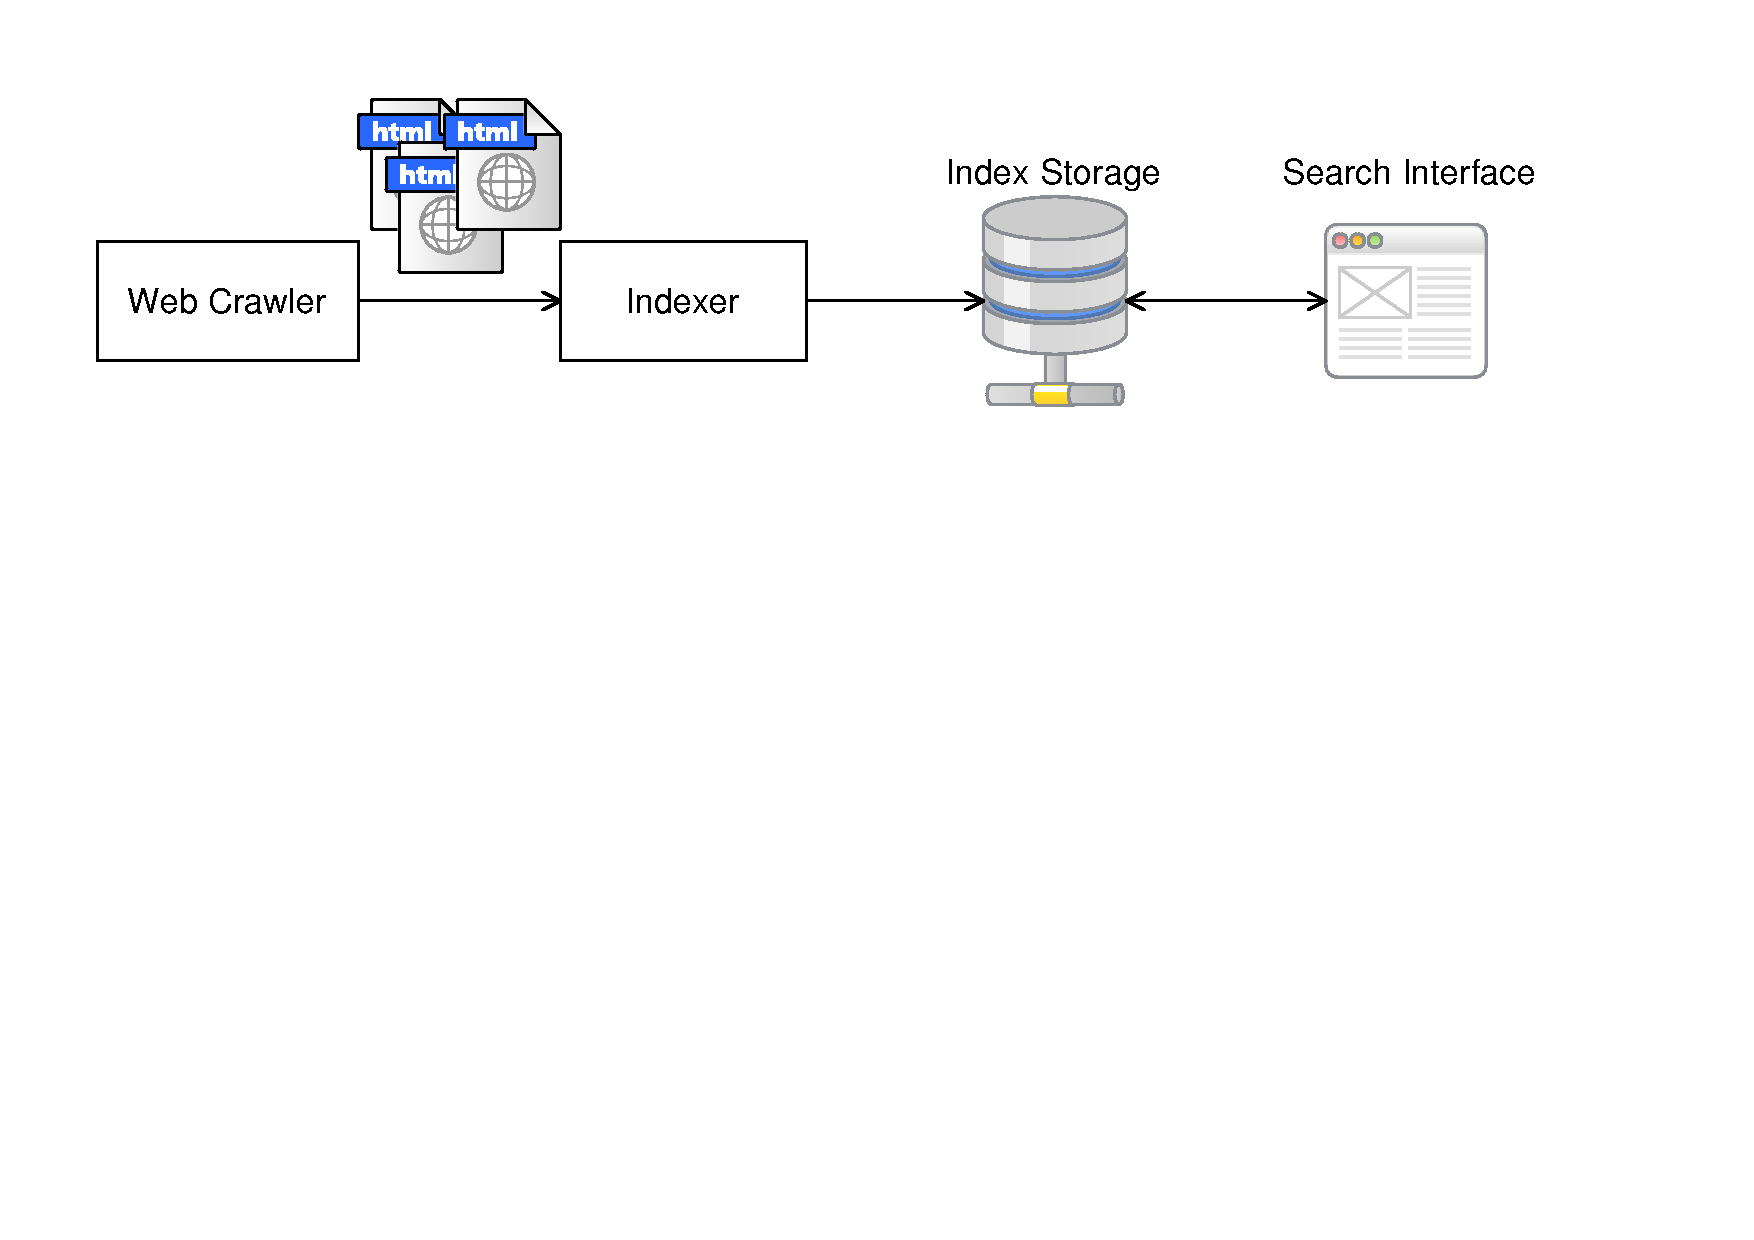
\includegraphics[scale=0.55, trim = 0mm 140mm 0mm 10mm,]{typical-se}
    \caption{A high-level architecture of a typical web search engine}
    \label{fig:web-search}
  \end{figure}

Web Crawler is a program that browses the World Wide Web reading the content of web pages in order to provide up-to-date data to Indexer. Indexer decides how a page content should be stored in an index storage. Indices help to quickly query documents from the index storage. Users can search and view query results through the Search Interface. When a user makes a query the search engine analyzes its index and returns best matched web pages according to specific criteria. 

Web crawlers that fetch web pages with the content in the same domain are called focused or topical crawlers \cite{chakrabarti1999focused}. An example of a focused crawler is an academic-focused crawler that crawls scientific articles. Such crawlers become components of focused search engines. Examples of popular academic search engines are Google Scholar and CiteSeer. Chapter \ref{cha:related-work} gives an overview of these search engines.  

\section{Inverted Index}
Search engines like CiteSeer or Google Scholar deal with a large collection of documents. The way to avoid linear scanning the text of all documents for each query is to \emph{index} them in advance. Thereby we are coming to the concept of \emph{inverted index}, which is a major concept in IR. The term \emph{inverted index} comes from the data structure storing a mapping from content, such as words or numbers, to the parts of a document where it occurs. Figure \ref{fig:inverted-index} shows the basic example of an inverted index. We have a dictionary of terms appearing in the documents. Each term maps to a list that records which documents the term occurs in. Each item in the list, conventionally named as \emph{posting}, records that a term appears in a document, often it records the position of the term in the document as well. The dictionary on Figure \ref{fig:inverted-index} has been sorted alphabetically and each postings list is sorted by document ID. Document ID is a unique number that can be assigned to a document when it is first encountered. \\
  \begin{figure}[htp]
    \centering
    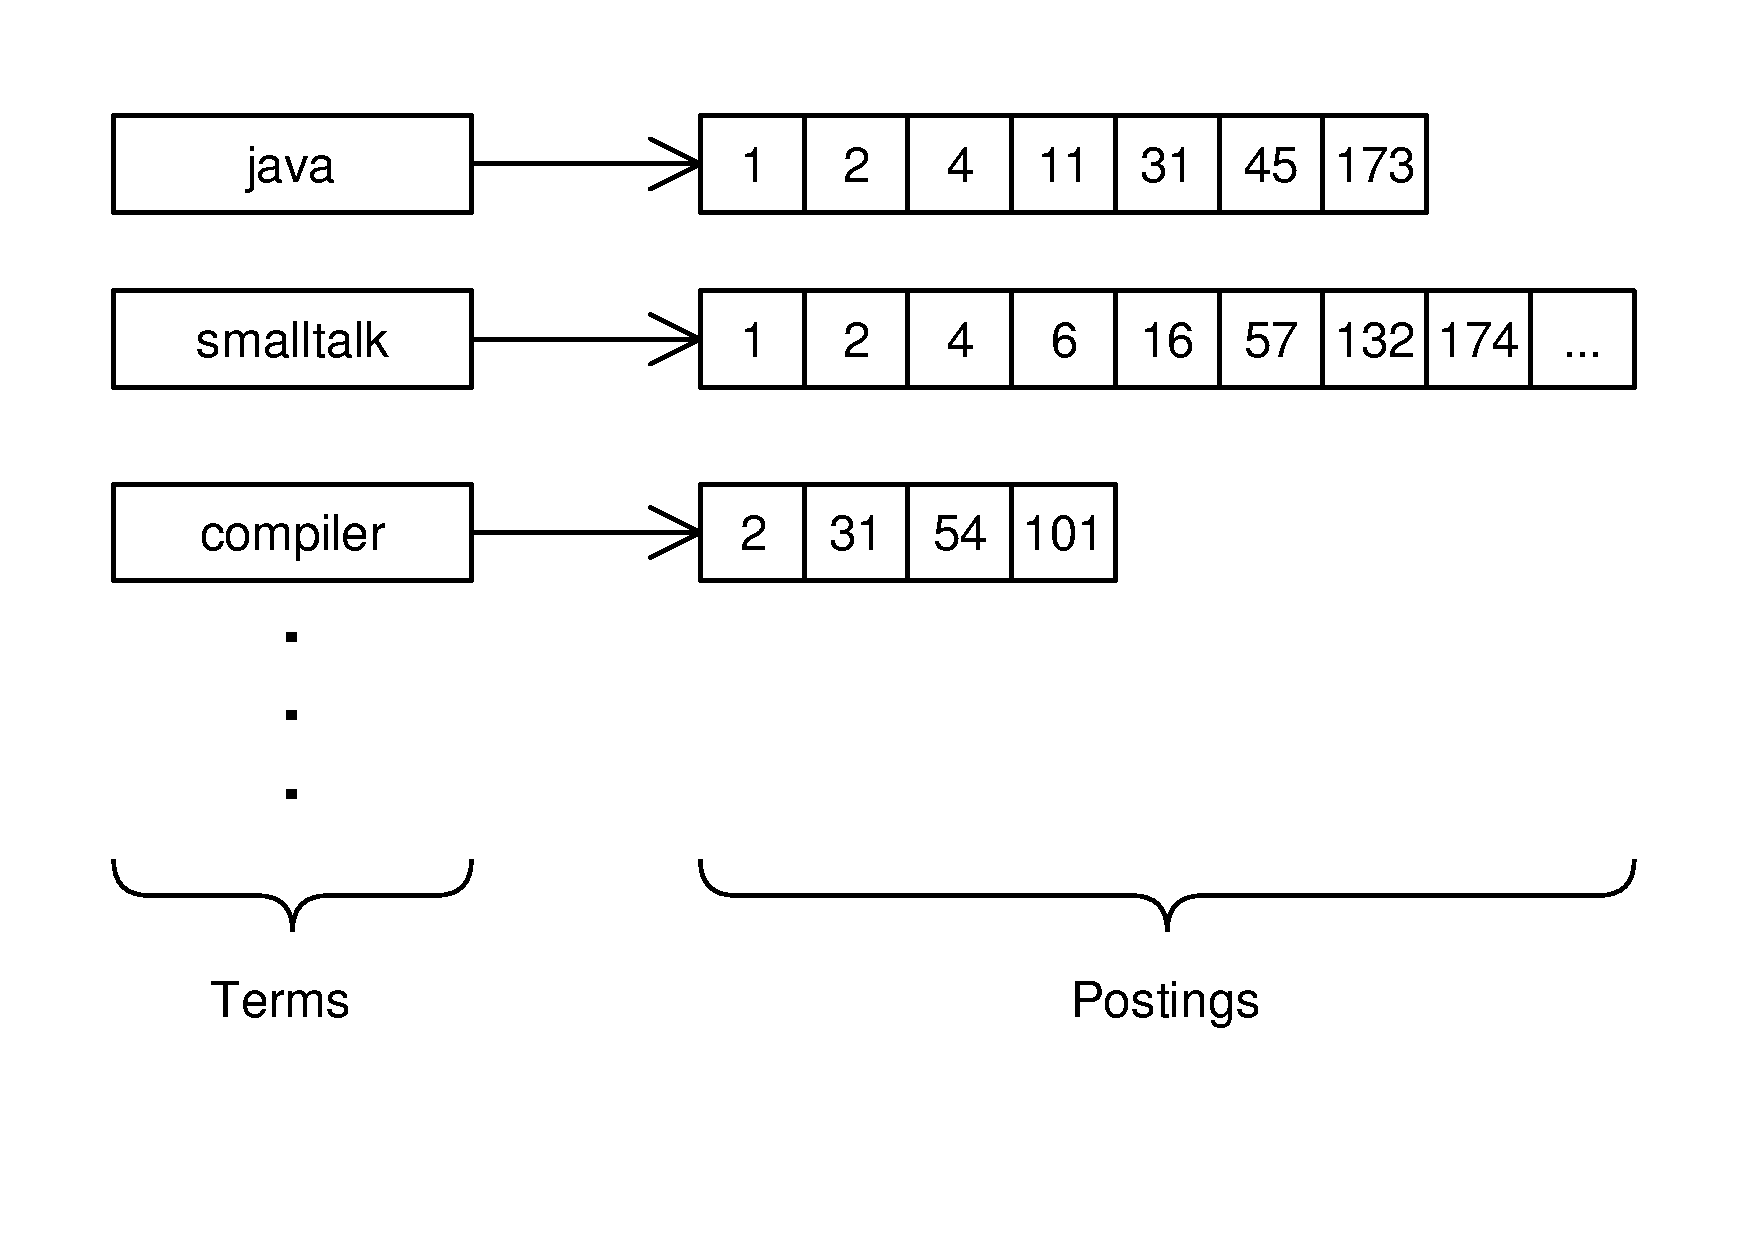
\includegraphics[scale=0.35, trim = 0mm 30mm 0mm 10mm]{inverted-index}
    \caption{Example of an inverted index. Each term in a dictionary maps to a posting list consisting of document IDs, where this term occurs. Dictionary terms are sorted alphabetically and posting lists are sorted by document IDs}
    \label{fig:inverted-index}
  \end{figure}
  
 The construction of the inverted index has following steps:
 
\begin{enumerate}
	\item Obtaining a document collection (usually performed by the crawler);
	\item Breaking each document into tokens, turning a document into a list of tokens;
  	\item Linguistic preprocessing of a list of tokens into normalized list of tokens;
	\item Index documents by creating an inverted index, consisting of a dictionary with terms and postings.
\end{enumerate}

First step of the index construction is obtaining a collection of documents. The goal here is to collect a set of documents containing textual data.
%Consider, for example, a collection of documents in PDF format \brs{why? we are talking about traditional search engines}.
%First, we need to correctly decode characters of the binary representation.
%Next, we should determine a document unit. For example, it might be a chapter in a book, or a paragraph in a scientific article. 

The next step is to break up each document into \emph{tokens}. Tokens can be thought of as the semantical units for processing. For example, it might be a word or a number. During tokenization, some characters, such as punctuation marks, can be thrown away. 

An example of the tokenization process is shown below:

\hspace{100pt}\textcolor[rgb]{0,0,1}{Input: Sometimes, I forget things.}

\hspace{100pt}\textcolor[rgb]{0,0,1}{Output: \framebox{Sometimes} \framebox{I} \framebox{forget} \framebox{things}} \\

The third step is normalization. Consider an example of querying the word \emph{co-operation}. A user might also be interested in getting documents containing \emph{cooperation}. \emph{Token normalization} is a process of turning a token into a canonical form so matches can occur despite lexical differences in the character sequences. One way of token normalization is keeping relations between unnormalized tokens, which can be extended to manual constructed synonym lists, such as \emph{car} and \emph{automobile}. The most standard way of token normalization however is creating \emph{equivalence classes}. If tokens become identical after applying a set of rules then they are in the equivalence classes. Consider the following common normalization rules that are often used:

\begin{description}
	\item[Stemming and Lemmatization] Words can be used in different grammatical forms. For instance, \emph{organize}, \emph{organizes}, \emph{organizing}.However in many cases it sounds reasonable for one of these words to return documents contain other forms of the word. The goal of stemming and lemmatization is to reduce the form of the word to a common base form. 
	
Here is an example: 
	
\hspace{100pt} \textcolor[rgb]{0,0,1}{ am, are, is = \textgreater be }

\hspace{100pt} \textcolor[rgb]{0,0,1}{car, cars, car's, cars'  =\textgreater car}

The result of applying the rule to the sentence:

\hspace{100pt} \textcolor[rgb]{0,0,1}{three frogs are flying   =\textgreater three frog be fly}

Stemming and lemmatization are closely related concepts however there is a difference. \emph{Lemmatization} usually refers to finding a \emph{lemma}, common base of a word, with the help of a vocabulary, morphological analysis of a word and requires understanding the context of a word and language grammar. \emph{Stemming} however operates with a word without knowing its context and thereby can't distinguish that the same words have different meanings depending on the context. 

Here is an example:

\hspace{10pt} \textcolor[rgb]{0,0,1}{ better = \textgreater good }, can only be matched by lemmatization since it requires dictionary look-up

\hspace{10pt} \textcolor[rgb]{0,0,1}{writing  =\textgreater write}, can be matched by both lemmatization and stemming

\hspace{10pt} \textcolor[rgb]{0,0,1}{meeting  =\textgreater meeting(noun) or to meet(verb)}, can be matched only by lemmatization since it requires the word context 

In general, stemmers are easier to implement and run faster. The most common algorithm for stemming is \emph{Porter's} algorithm \cite{Porter:1997:ASS:275537.275705}.
	  
	\item[Capitalization/Case-Folding] A simple strategy is to reduce all letters to a lower case, so that sentences with \emph{Automobile} will match to queries with \emph{automobile}. However this approach would not be appropriate in some contexts like identifying company names, such as \emph{General Motors}. Case-folding can be be done more accurately by a machine learning model using more features to identify whether a word should be lowercased.
	\item[Accents and Diacritics]  Diacritics in English language play an insignificant role and simply can be removed. For instance \emph{clich\'e} can be substituted by \emph{cliche}. In other languages diacritics can be part of the writing system and distinguish different sounds. However, in many cases, users can enter queries for words without diacritics.
\end{description}

The last step of building the inverted index is sorting. The input to indexing is a list of pairs of normalized tokens and documents IDs for each document. Consider an example of three documents with their contents:
\begin{itemize}
	\item Document 1: Follow the rules.
	\item Document 2: This is our town.
	\item Document 3: The gates are open.
\end{itemize}

 After applying tokenization and normalization steps of the listed documents the input to the indexing is shown in Table \ref{tab:input-indexing}. 
\begin{table}[ht]
\begin{center}
\begin{tabular}{ | l | l | } 
 \hline
 \textbf{Term} & \textbf{DocumentID} \\  \hline
 follow & 1\\ 
 the & 1\\
 rule & 1\\
 this & 2\\ 
 be & 2\\
 our & 2\\
 town & 2\\
 the & 3\\ 
 gate & 3\\
 be & 3\\
 open & 3\\        
 \hline
\end{tabular}
\caption{Input to the indexing algorithm is a list of pairs of a term and document ID, where this term occurs.}
\label{tab:input-indexing}
\end{center}
\end{table}
The indexing algorithm sorts the input list so that the terms are in alphabetical order as in Table \ref{tab:indexing-sorting}. 
 \begin{table}[ht]
\begin{center}
\begin{tabular}{ | l | l | } 
 \hline
 \textbf{Term} & \textbf{DocumentID} \\  \hline
 be & 2\\ 
 be & 3\\
 follow & 1\\
 gate & 3\\
 open & 3\\
 our & 2\\
 rule & 1\\
 the & 1\\
 the & 3\\
 this & 2\\
 town & 2\\   
 \hline
\end{tabular}
\caption{Indexing algorithm sorts all terms in a alphabetical order. The result is a list of sorted terms with document IDs}
\label{tab:indexing-sorting}
\end{center}
\end{table}
Then it merges the same terms from the same document by folding two identical adjacent items in the list. And finally instances of the same term are grouped and the result is split into a dictionary with postings, as shown in Table \ref{tab:indexing-merging}.
 \begin{table}[ht]
\begin{center}
\begin{tabular}{ | l | l | } 
 \hline
 \textbf{Term} & \textbf{Postings} \\  \hline
 be & 2 3\\ 
 follow & 1\\
 gate & 3\\
 open & 3\\
 our & 2\\
 rule & 1\\
 the & 1 3\\
 this & 2\\
 town & 2\\   
 \hline
\end{tabular}
\caption{Indexing algorithm groups the same terms with creating postings. The result is a dictionary with terms as keywords and values as postings.}
\label{tab:indexing-merging}
\end{center}
\end{table}


%%Since a term generally occurs in a number of documents, this data organization already reduces the storage requirements of the index. 

\section{Dynamic Indexing}
So far we assumed that document collection is static. However there are many cases when the collection can be updated, for example, by adding new documents, deleting or updating existing documents. Simple way to deal with dynamic collection is to reconstruct the inverted index from scratch. This might be acceptable if the changes made in the collection are small over time and the delay in making new documents searchable is not critical. However if there is one of the aforementioned conditions is violated, one might be interested in another more dynamic solution like keeping an auxiliary index. Thus we have a large main index and we keep auxiliary index for changes. The auxiliary index is kept in memory. Every time a user makes a query the search runs over both indexes and results are merged. When the auxiliary index becomes too large it can be merged with the main index.

\section{Retrieving Search Results}
When a user makes a query it would be good to give her back a result document containing all terms in the query, so that terms are located close to each other in the document. Consider an example of querying a phrase containing 4 terms. The part of the document that contains all terms is named a \emph{window}. The size of the window is measured in number of words. For instance the smallest window for 4-term query will be 4. Intuitively, smaller windows represent better results for users. Such a window can become one of the parameters ranking a document in the search result. If there is no document containing all 4 terms, a 3-term phrase can be queried. Usually search systems hide the complexity querying from the user by introducing \emph{free text query parsers} so a user can make only one query.

\chapter {Related Work}
\label{cha:related-work}

\section{Citations In Scientific Publications}

Citations are the subject of many interesting scientific studies. 

Bradshaw et al. \cite{bradshaw} showed that citations provide many different perspectives on the same article. They believe that citation provide means to measure the relative impact of articles in a collection of scientific literature. In their work the authors improved the relevance of documents in the search engine results with a method called Reference Directed Indexing. Reference Directed Indexing (RDI) is based on a comparison of the terms authors use in reference to documents.

Bertin and Atanassova \cite{marc1} \cite{M_automaticannotation} \cite{autocit} automatically extract citations and annotate them using a set of semantic categories. In \cite{M_automaticannotation} and \cite{marc1} they used linguistic approach, which used the contextual exploration method, to annotate
automatically the text. In \cite{autocit} they proposed a hybrid method for the extraction and characterization of citations in scientific papers using machine learning combined with rule-based approaches. 

There are several studies that used citations to evaluate science by introducing map of science. Map of science graphically reflects the structure, evolution and main contributors of a given scientific field \cite{map1} \cite{Klavans:2009:TCM:1527090.1527095} \cite{DBLP:journals/corr/abs-1202-1914} \cite{Small:1999:VSC:308915.308932}. 

Kessler \cite{ASI:ASI5090140103} first used the concept of bibliographic coupling for document clustering. To build a cluster of similar documents Kessler used a similarity function based on the degree of bibliographic coupling. Bibliographic coupling is a number of citations two documents have in common. The idea was developed further by Small in co-citation analysis \cite{ASI:ASI4630240406}. Later co-citation analysis and bibliographic coupling was used by Larson \cite{larson1996bibliometrics} for measuring similarity of web pages.

Another approach is to use citations to build summaries of scientific publications. There are three categories of summaries proposed based on citations: overview of a research area (multi-document summarization) \cite{Nanba:1999:TMS:1624312.1624351}, impact summary (single document summary with citations from the scientific article itself) \cite{mei-zhai:2008:ACLMain} and citation summary (multi- and single document summarization, in which citations from other papers are considered) \cite{Qazvinian:2008:SPS:1599081.1599168}. In work by Nakov et al. citations have been used to support automatic paraphrasing \cite{Nakov04citances:citation}. 

An expert literature survey on citation analysis was made by Smith \cite{smith}, she reviewed hundred of scientific articles on this topic. 

\section{Popular Academic Search Engines}
\paragraph{CiteSeer\textsuperscript{x}}

CiteSeer\textsuperscript{x} is built on the concept of citation index. The concept of citation index was first introduced by Eugene Garfield in \cite{garfield1964science}. In terms of Eugene Garfield citations are bibliographic links or referrers linking scientific documents. In his work Eugene Garfield proposed an approach where citations between documents were manually cataloged and maintained so that a researcher can search through listings of citations traversing citation links either back through supporting literature or forward through the work of later researchers \cite{bradshaw2002reference}.

Lawrence et al. automated this process in CiteSeer\textsuperscript{x} \footnote{CiteSeer, \url{http://citeseerx.ist.psu.edu/}} \cite{Giles:1998:CAC:276675.276685}, a Web-based information system that permits users to browse the citation links between documents as hyperlinks. CiteSeer\textsuperscript{x} automatically parses and indexes publicly available scientific articles found on the World Wide Web. 

CiteSeer\textsuperscript{x} is built on top of the the open source infrastructure SeerSuite \footnote{SeerSuite, \url{http://citeseerx.sourceforge.net/}} and uses Apache Solr \footnote{Apache Solr. \url{http://lucene.apache.org/solr/}} search platform for indexing documents. It can extract meta information from papers such as title, authors, abstract, citations. The extraction methods are based on machine learning approaches such as ParseCit \cite{Councill08parscit:an}. 
CiteSeer\textsuperscript{x} currently has over 4 million documents with nearly 4 million unique authors and 80 million citations. 

CiteSeer\textsuperscript{x} indexes citations more precisely bibliographic links or referrers while in CiteWise we intend to index not only bibliographic links but also cited text in a body of a document. If by indexing bibliographic links CiteSeer\textsuperscript{x} mainly aims to simplify navigation between linked documents, in CiteWise we focus on simplifying retrieval of documents containing a text of interest.  
\\ \\
\textbf{Google Scholar} 
Google Scholar is a freely accessible web search engine that makes full-text or metadata indexing of scientific literature \footnote{Google Scholar, \url{http://scholar.google.ch/}}. Besides the simple search Google Scholar proposes following features: unique ranking algorithm, an algorithm that ranks documents ``the way researchers do, weighing the full text of each document, where it was published, who it was written by, as well as how often and how recently it has been cited in other scholarly literature'' \footnote{\url{https://scholar.google.com/scholar/about.html}}; "Cited by" feature allows to view abstracts of articles citing the given article; "Related articles" feature shows the list of closely related articles. It is also possible to filter articles by author name or published date.
Google Scholar contains roughly 160 million of documents by May 2014 \cite{orduna2014size}. 

%In which we understand what the problem is in detail.

\chapter {CiteWise}
\label{cha:CS}

\section{System Overview}

The components of CiteWise is shown on Figure \ref{fig:cs}. There are three main operations performed by CiteWise: parsing PDF files, indexing documents and querying the resulted indexes. Correspondingly, there are three major components responsible for accomplishment of these operations: \emph{Parser}, \emph{Indexer} and \emph{Search Web App}. The system has two more components for storing data: \emph{Indexes Storage} and \emph{Meta Data Storage}. We use \emph{Indexes Storage} for storing indexes built on citations. This storage is very simple and was not designed to represent any relations in data structures. Moreover, it does not allow to perform any sophisticated operations over the stored data. Therefore, we use \emph{Meta Data Storage} to represent complex data structures and perform sophisticated queries, like aggregating citations referring to the same article. 

  \begin{figure}[htp]
    \centering
    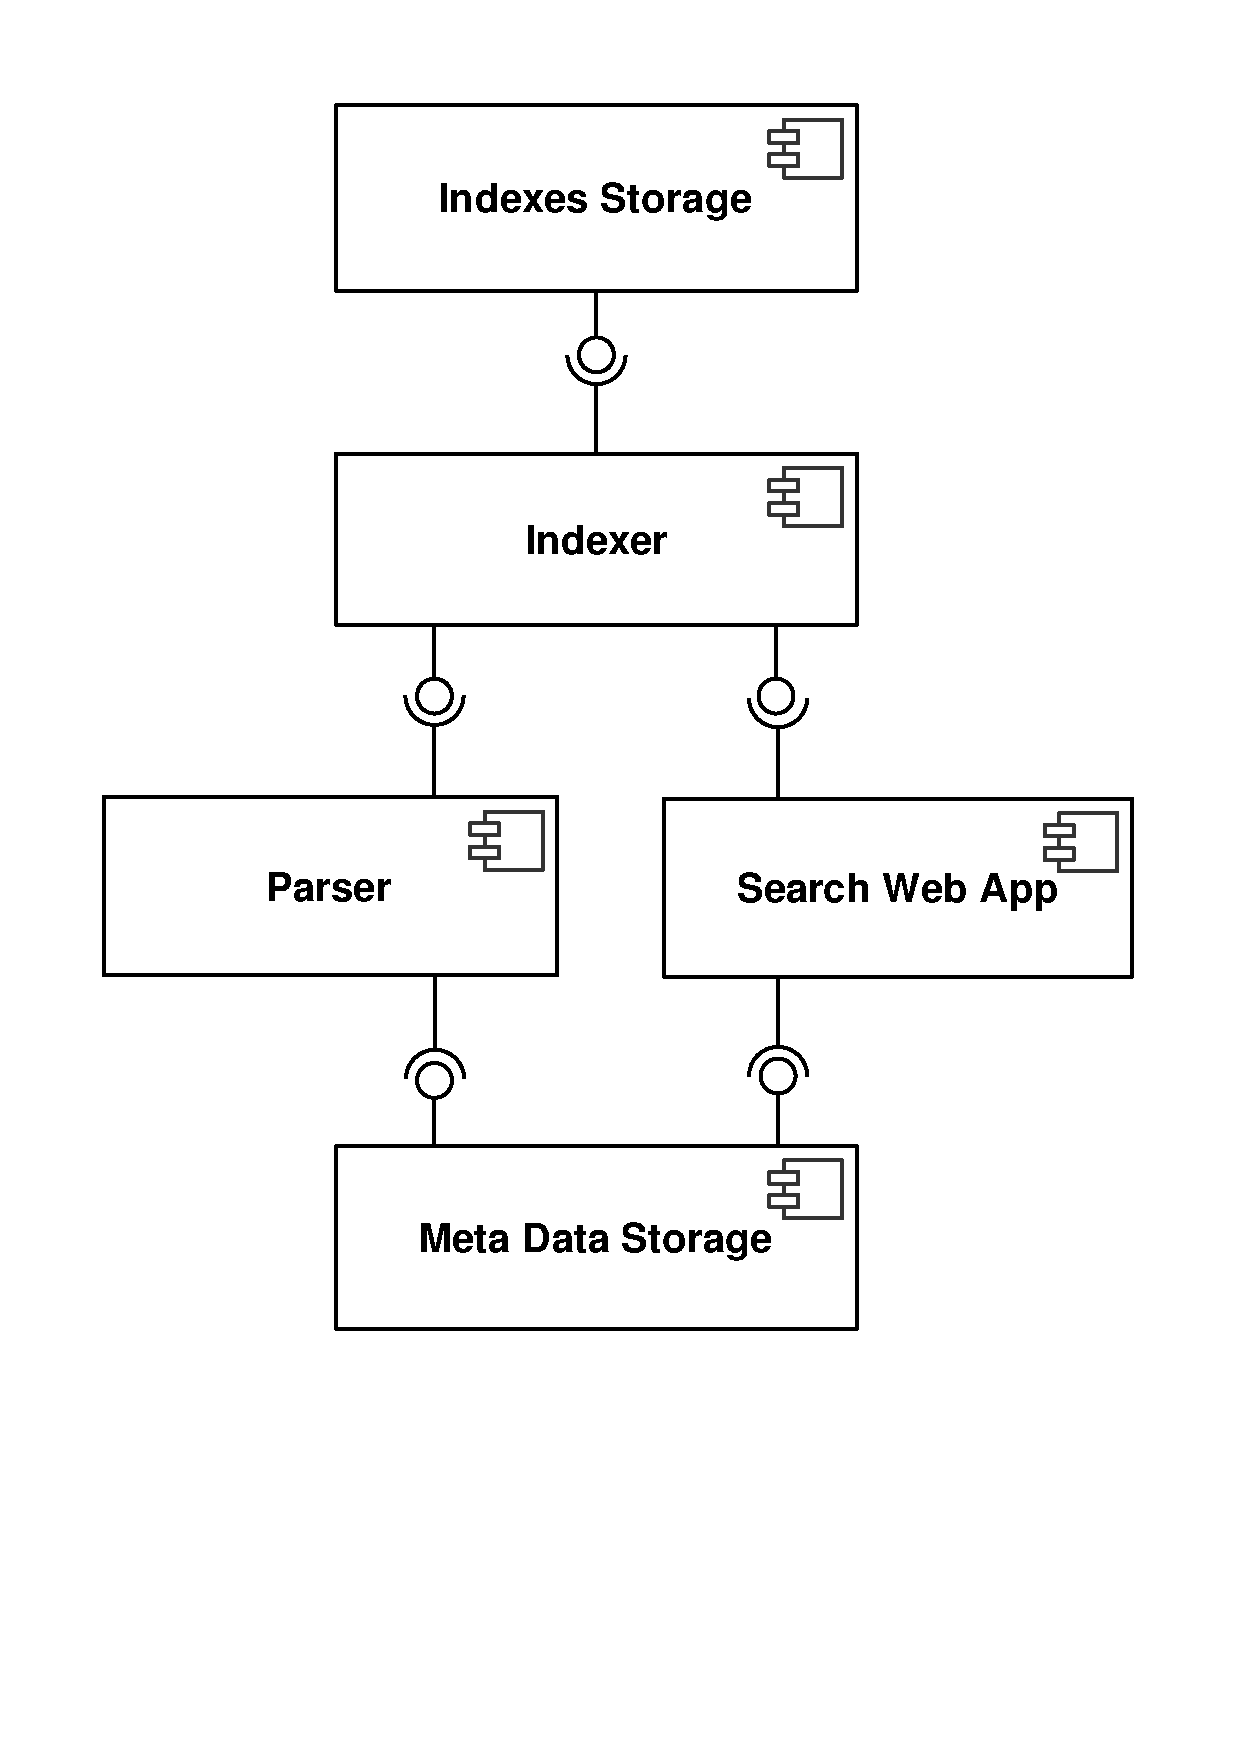
\includegraphics[scale=0.38, trim = 0mm 65mm 0mm 20mm]{cs-components}
    \caption{Component diagram of CiteWise.}
    \label{fig:cs}
  \end{figure}


The workflow of the system is shown on Figure \ref{fig:cs-activity-diagram}. The first operation performed by the system is parsing. The \emph{Parser} converts a PDF file into the text. Then it extracts meta information, like citations and references, from the textual representation of the file. Next it packages extracted information into data units corresponding to formats acceptable by \emph{Indexer} and \emph{Meta data storage}. A data unit publishable to the \emph{Indexer} consist of a citation, that should be indexed and an additional information related to this citation (citation context, a file URI, bibliographic references) that should be stored. A data unit publishable to the \emph{Meta data storage} consist of a citation, a source paper identifier and bibliographic references. We use \emph{Meta data storage} for aggregating citations referring to the same source. Once the \emph{Parser} processed the PDF file it can proceed to the next paper if there is any left. When all papers are processed, user can make queries over \emph{Search Web App}.

  \begin{figure}[htp]
    \centering
    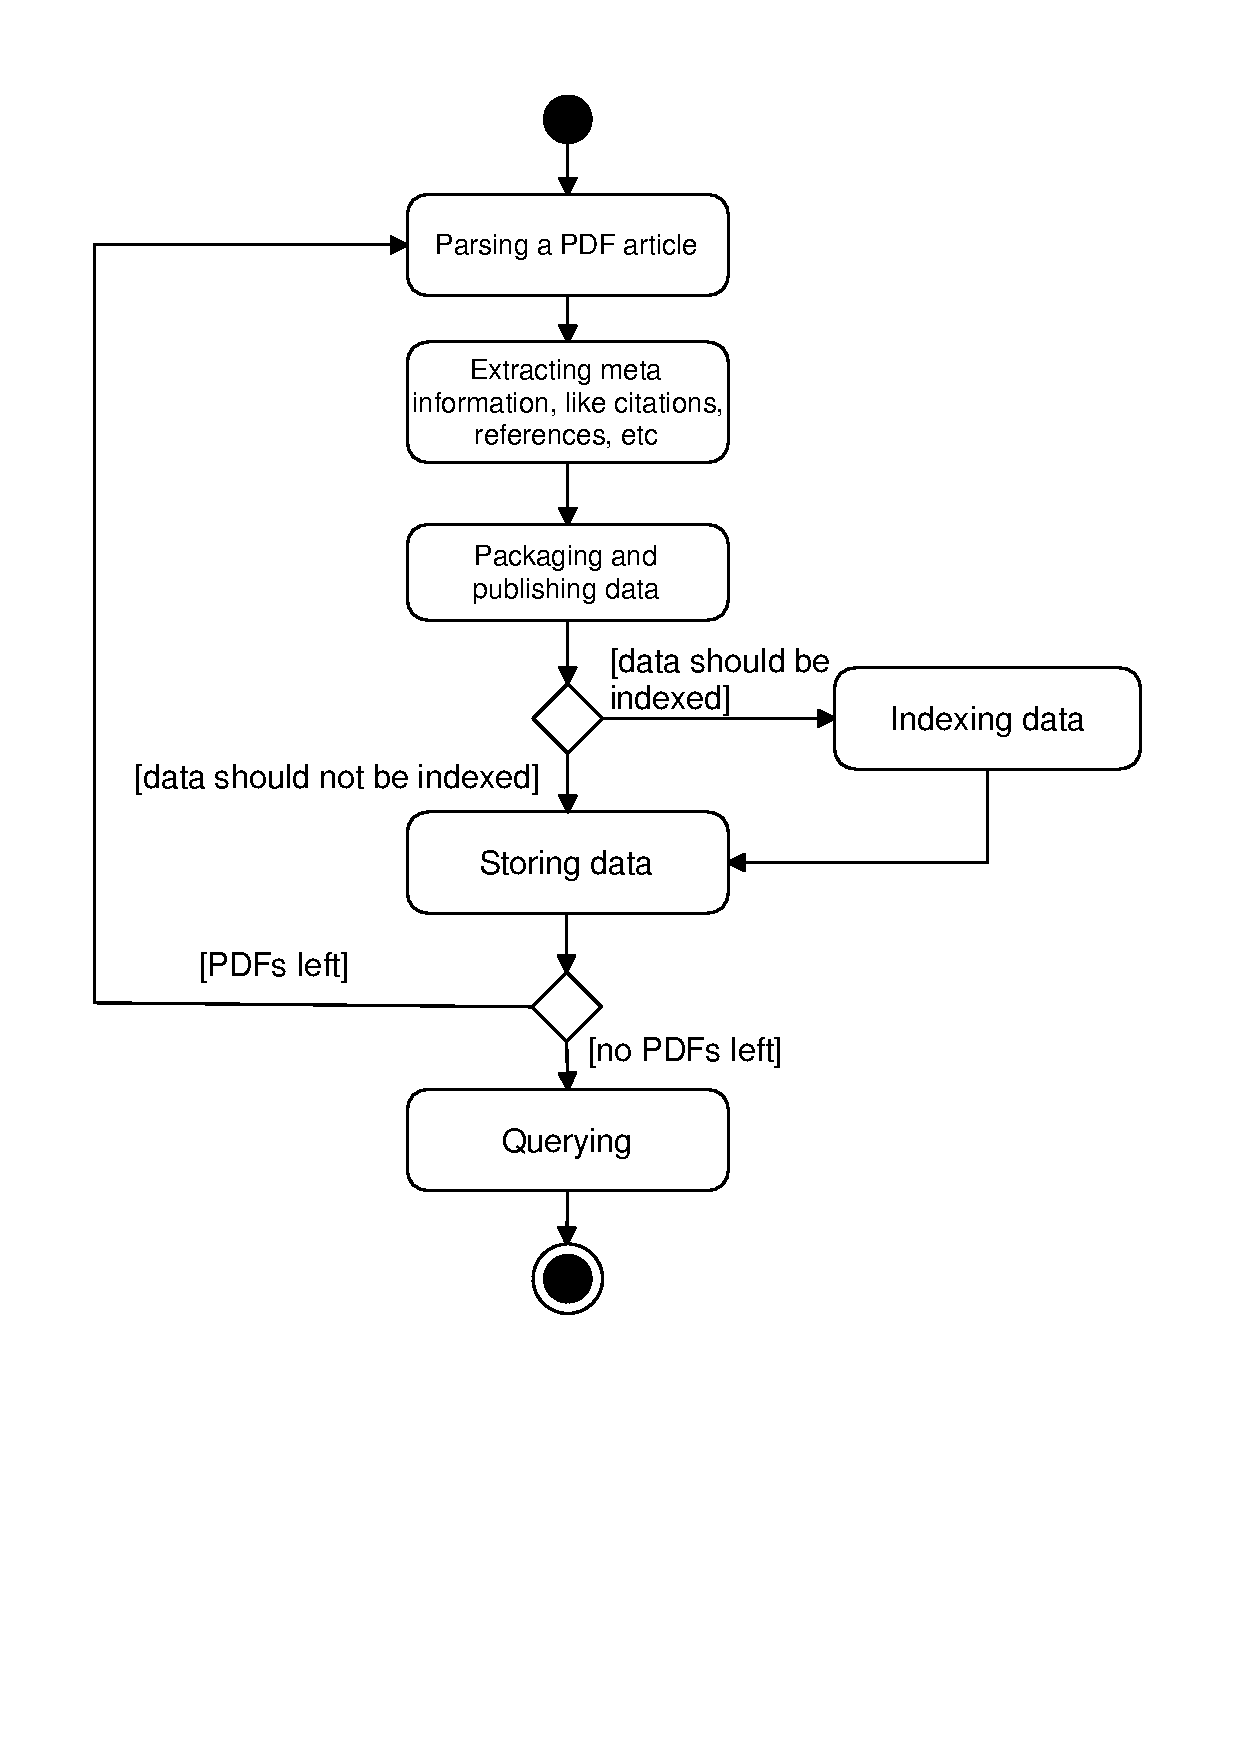
\includegraphics[scale=0.5, trim = 0mm 70mm 0mm 20mm]{cs-activity-diagram}
    \caption{Activity diagram of CiteWise.}
    \label{fig:cs-activity-diagram}
  \end{figure}

The next sections of this chapter describe the implementation of each component in detail and show the reasons behind choosing a particular solution.       

\section{Parser}

It is practical to divide the work of the \emph{Parser} into two phases: \emph{PDF processing} and \emph{Document publishing}, as in Figure \ref{fig:parser}. The output of the \emph{PDF processing} phase is the input to the \emph{Documents publishing} phase. 

  \begin{figure}[htp]
    \centering
    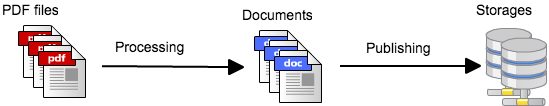
\includegraphics[scale=0.5, trim = 0mm 140mm 0mm 10mm]{parser}
    \caption{Parser workflow}
    \label{fig:parser}
  \end{figure}

\subsection{PDF Processing}
The main role of \emph{PDF processing} phase is to parse scientific articles into text and extract citations and bibliographic references to create documents for publishing. 
Parsing PDF-files from different sources is a very challenging task as there is a large number of scientific articles in different formats. 
%Besides that, there exist scientific articles written decades ago which can use different encoding algorithms\brs{not sure what this means, can you elaborate a bit?} from articles created recently. 
Thereby, building a universal parser is very hard in practice. In our case, we try to identify common patterns covering the majority of the scientific article formats or at least the formats found in our collection of articles.  

\emph{PDF processing} phase starts with recursively walking though the directory tree of the collection of PDF documents. While walking through the directory, the \emph{Parser} filters non-pdf files and parses and processes each PDF-file separately. We use Apache PDFBox library\footnote{Apache PDFBox, \url{https://pdfbox.apache.org/}}. The library extracts full text from PDF-files, but without any hints on the initial structure of the article. In our case, to find citations and bibliographic references in text, we need to look them up in different parts of the article. We designed an algorithm to break the PDF-text into sections.

Generally, we are interested in identifying a body of the document where we can find citations and reference blocks where we can find bibliographic links. One way of finding these sections can be using keywords that might signify the beginning or the end of some sections. Based on those keywords, one can extract different sections of a document. Figure \ref{fig:template} shows a sample text of a parsed pdf-document with keywords. 
  
One can notice the following characteristics of scientific articles:
\begin{itemize}
	\item The body of a document comes before the references section.
	\item The appendix or author's biography sections can come after the references section.
	\item Each document contains the ``Abstract" and the ``References" words and might contain the ``Appendix" word. We call these words keywords. 
\end{itemize}  

The keywords can be written in different formats, like using upper or lower cases. Table \ref{tab:keywords} illustrates some variations of the keywords.

\begin{table}[ht]
\begin{center}
\begin{tabular}{ | l | l | l | } 
 \hline
 body & references & appendix \\  \hline
 Abstract & References & Appendix \\ 
 ABSTRACT & References: & APPENDIX \\
 & REFERENCES & \\  
 \hline
\end{tabular}
\caption{Keywords identifying different sections in a document}
\label{tab:keywords}
\end{center}
\end{table}

After breaking a document down into sections as shown in Figure \ref{fig:template}, the text is presented in one-column format. There are two aspects regarding this format. First, sentences can be split by new line symbols at the end of a line. Second, words can be split by dash symbol at the end of a line. We introduce a normalization step where new lines are substituted by white spaces and dashes are removed in the end of a line to obtain continuous text.

  \begin{figure}[htp]
  	\centering
    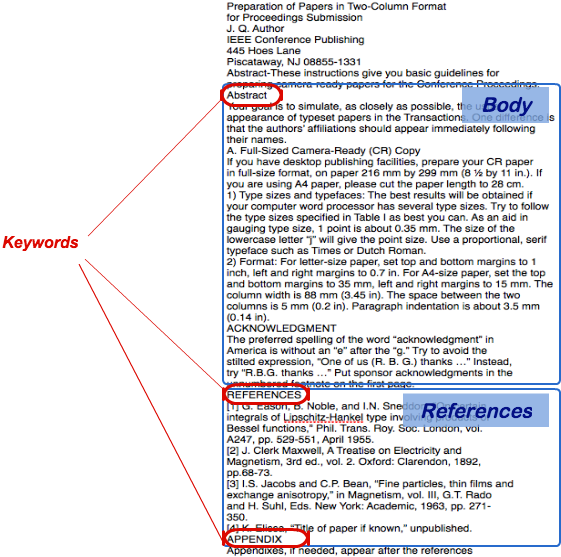
\includegraphics[scale=0.6, trim = 50mm 0mm 0mm 0mm]{template}
    \caption{Sample text of the parsed scientific article. Keywords help to break the document into sections.}
    \label{fig:template}
  \end{figure}

As a result of the normalization step, we have a document divided into body and references sections. Before searching citations in the body of a document, we break the body into sentences. In general, breaking text into sentences is not an easy task. Consider a simple example with a period. Period not only indicates the end of a sentence but also can be encountered inside the sentence itself, like an item of a numbered list or a name of a scientist. Besides, not all sentences end with a period, like the title of a section or an item of a list. We use Stanford CoreNLP library that employs natural language and machine learning techniques to extract sentences \cite{stanford.nlp}. 

Next, we search for the citations in the body and for the bibliography links in the references section. When an author makes a citation she puts a link to a bibliographic reference in the sentence. It is common to use square brackets ([ and ]) to make a link to a bibliographic reference in the sentence. Thus, we can identify citations by detecting square brackets in the text. After analyzing some set of articles we found multiple patterns in using square brackets for {citations, as shown in Table \ref{tab:citations}. 

\begin{table}[ht]
\begin{center}
\begin{tabular}{ | l | p{7cm} | } 
 \hline
 Patterns of using [ ] & Example in text \\  \hline
 {[}21{]} & Our conclusion is that, contrary to prior pessimism \textbf{[21]}, [22], data mining static code attributes to learn defect predictors is useful. \\ \\ 
 {[}20, 3, 11, 17{]} & In the nineties, researchers focused on specialized multivariate models, i.e., models based on sets of metrics selected for specific application areas and particular development environments \textbf{[20, 3, 11, 17]}. \\ \\
 {[}24, Sections 6.3 and 6.4 {]}& Details on the life-cycle of a bug can be found in the BUGZILLA documentation \textbf{[24, Sections 6.3 and 6.4]}. \\ \\
 {[}PJe02{]} & In a lazy language like Haskell \textbf{[PJe02]} this is not an issue - which is one key reason Haskell is very good at defining domain specific languages.  \\ \\
 \hline
\end{tabular}
\caption{Frequent patterns in using square brackets ([ and ])for citing}
\label{tab:citations}
\end{center}
\end{table}


Further we need to extract bibliographic links from the references section. For that we studied most common variants of composing the references sections. Table \ref{tab:references} summarises these findings. To extract bibliographic links we make a list of regular expressions matching one of those patterns listing in Table \ref{tab:references}. Extracting bibliographic links allows us to match citations with bibliographic links.

\begin{table}[h]
\begin{center}
\begin{tabular}{ | p{12cm} | } 
 \hline
 References section templates\\  \hline
 \textbf{[1]} J. Bach. Useful features of a test automation system (partiii) \ldots \newline
 \textbf{[2]} B. Beizer. Black-Box Testing. John Wiley and Sons, \ldots \newline
 \ldots \\ \hline 
 \textbf{1.}  J. R. Hobbs,  Granularity, Ninth International Joint Conference \ldots \newline
  \textbf{2.}  W. Woods, What's in a Link:  Foundations for Semantic Networks, \ldots \newline
  \ldots \\ \hline
  \textbf{[1].}   Arnold, R.S., Software Reengineering, ed. \ldots \newline
  \textbf{[2].}   Larman, C., Applying  UML and Patterns. 1998, \ldots \newline  
  \ldots \\ \hline
  \textbf{[ASU86]} A. V. Aho, R. Sethi, and J. D. Ullman. Compilers: \ldots \newline
  \textbf{[AU73]} A.V. Aho and J.D. Ullman. The theory of parsing, translation \ldots \newline 
  \ldots \\
 \hline
\end{tabular}
\caption{Frequent patterns of writing bibliographic links in a references block}
\label{tab:references}
\end{center}
\end{table}

The pipeline of PDF processing stages described above is depicted on Figure \ref{fig:proc}. As seen from Figure \ref{fig:proc} to complete the processing stage we need to perform one more step: extracting titles from bibliographic links. The objective point of extracting titles from bibliographic links is to collect citations referring to the the same source (scientific article). In general case, different formats of bibliographic links can identify the same source or scientific article. For example, an article may have different editions, published in different journals in different years or simply different authors may use different style formatting. What we consider to be identical for all bibliographic links citing the same paper is the paper's title.   

  \begin{figure}[htp]
    \centering
    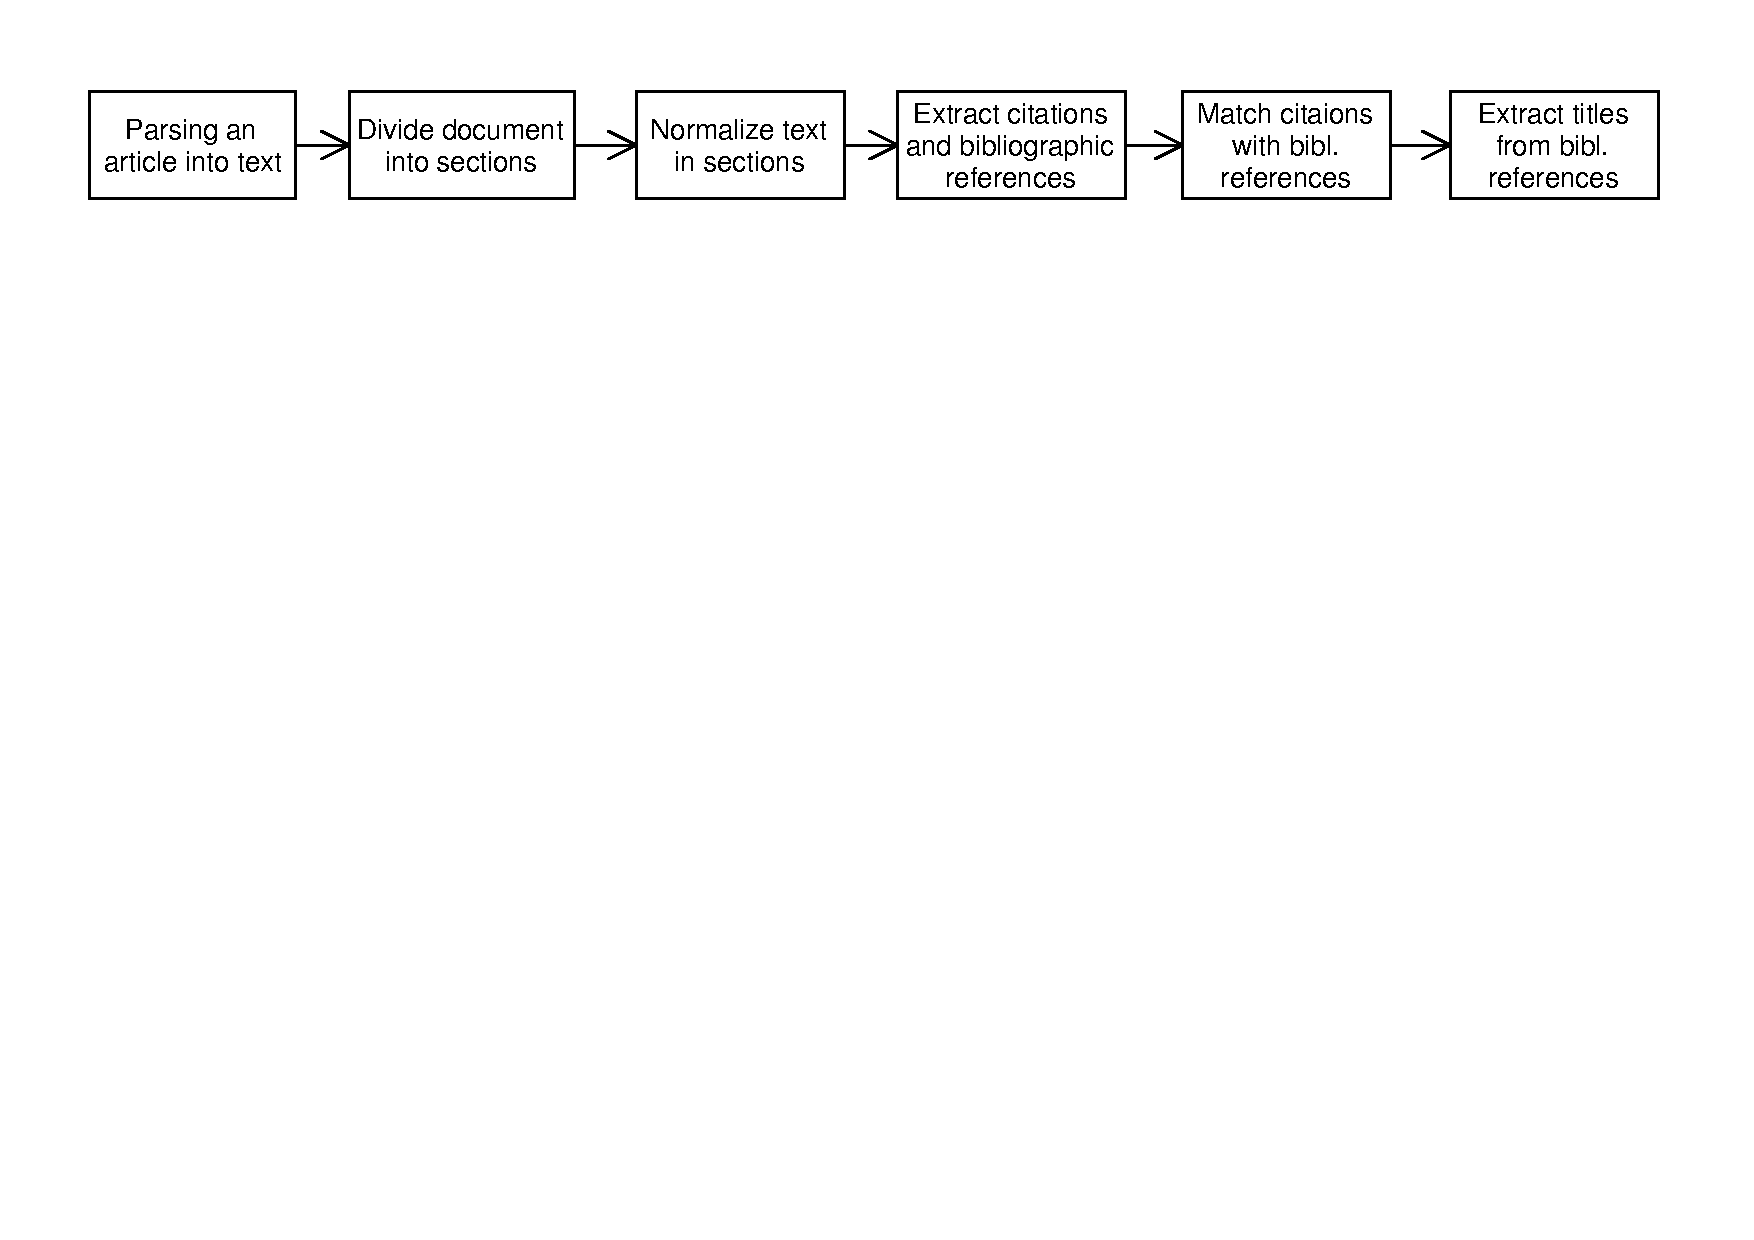
\includegraphics[scale=0.5, trim = 0mm 165mm 0mm 10mm]{processing}
    \caption{Pipeline of the PDF processing stage}
    \label{fig:proc}
  \end{figure} 

\paragraph{Processing bibliographic links}
We try to recognize common patterns covering the majority of bibliographic links. Table \ref{tab:bibl.links} shows some examples of bibliographic links. First,we noticed that if a bibliographic link contains some sort of quotation marks, for example, double quotes (``'') or single quotes (`'), then it is highly probable that a title is enclosed by these quotes. Then, we made some observations for bibliographic links without quotes. Very often, a bibliographic link is structured as follows: it begins by listing the paper's authors, then the title, and then comes the rest of the link (see Figure \ref{fig:link}). We use Core NLP library to break a link into parts according to our view. In most of cases it is enough to take the second part of the bibliographic link to be a title.

\begin{table}[h]
\begin{center}
\begin{tabular}{ | p{12cm} | } 
 \hline
 Conradi, R., Dyba, T., Sjoberg, D.I.K., and Ulsund, T., "Lessons learned and recommendations from two large norwegian SPI programmes." Lecture notes in computer science, 2003, pp. 32-45."
 \\ \hline 
 P. Molin, L. Ohlsson, `Points \& Deviations - A pattern language for fire alarm systems,' to be published in Pattern Languages of Program Design 3, Addison-Wesley.
 \\ \hline
  R. P. Wilson and M. S. Lam. Effective context sensitive pointer analysis for C programs. In PLDI, pages 1–12, June 1995. 289 
  \\ \hline
  Allen, Thomas B. Vanishing Wildlife of North America. Washington, D.C.: National Geographic Society, 1974.
  \\ \hline
  I. Herraiz, J. M. Gonzalez-Barahona, and G. Robles. Towards a Theoretical Model for Software Growth. In Proceedings of the 4th International Workshop on Mining Software Repositories, Minnesotta, USA, May 2007.
  \\
 \hline
\end{tabular}
\caption{Some examples of bibliographic links}
\label{tab:bibl.links}
\end{center}
\end{table}

  \begin{figure}[htp]
    \centering
    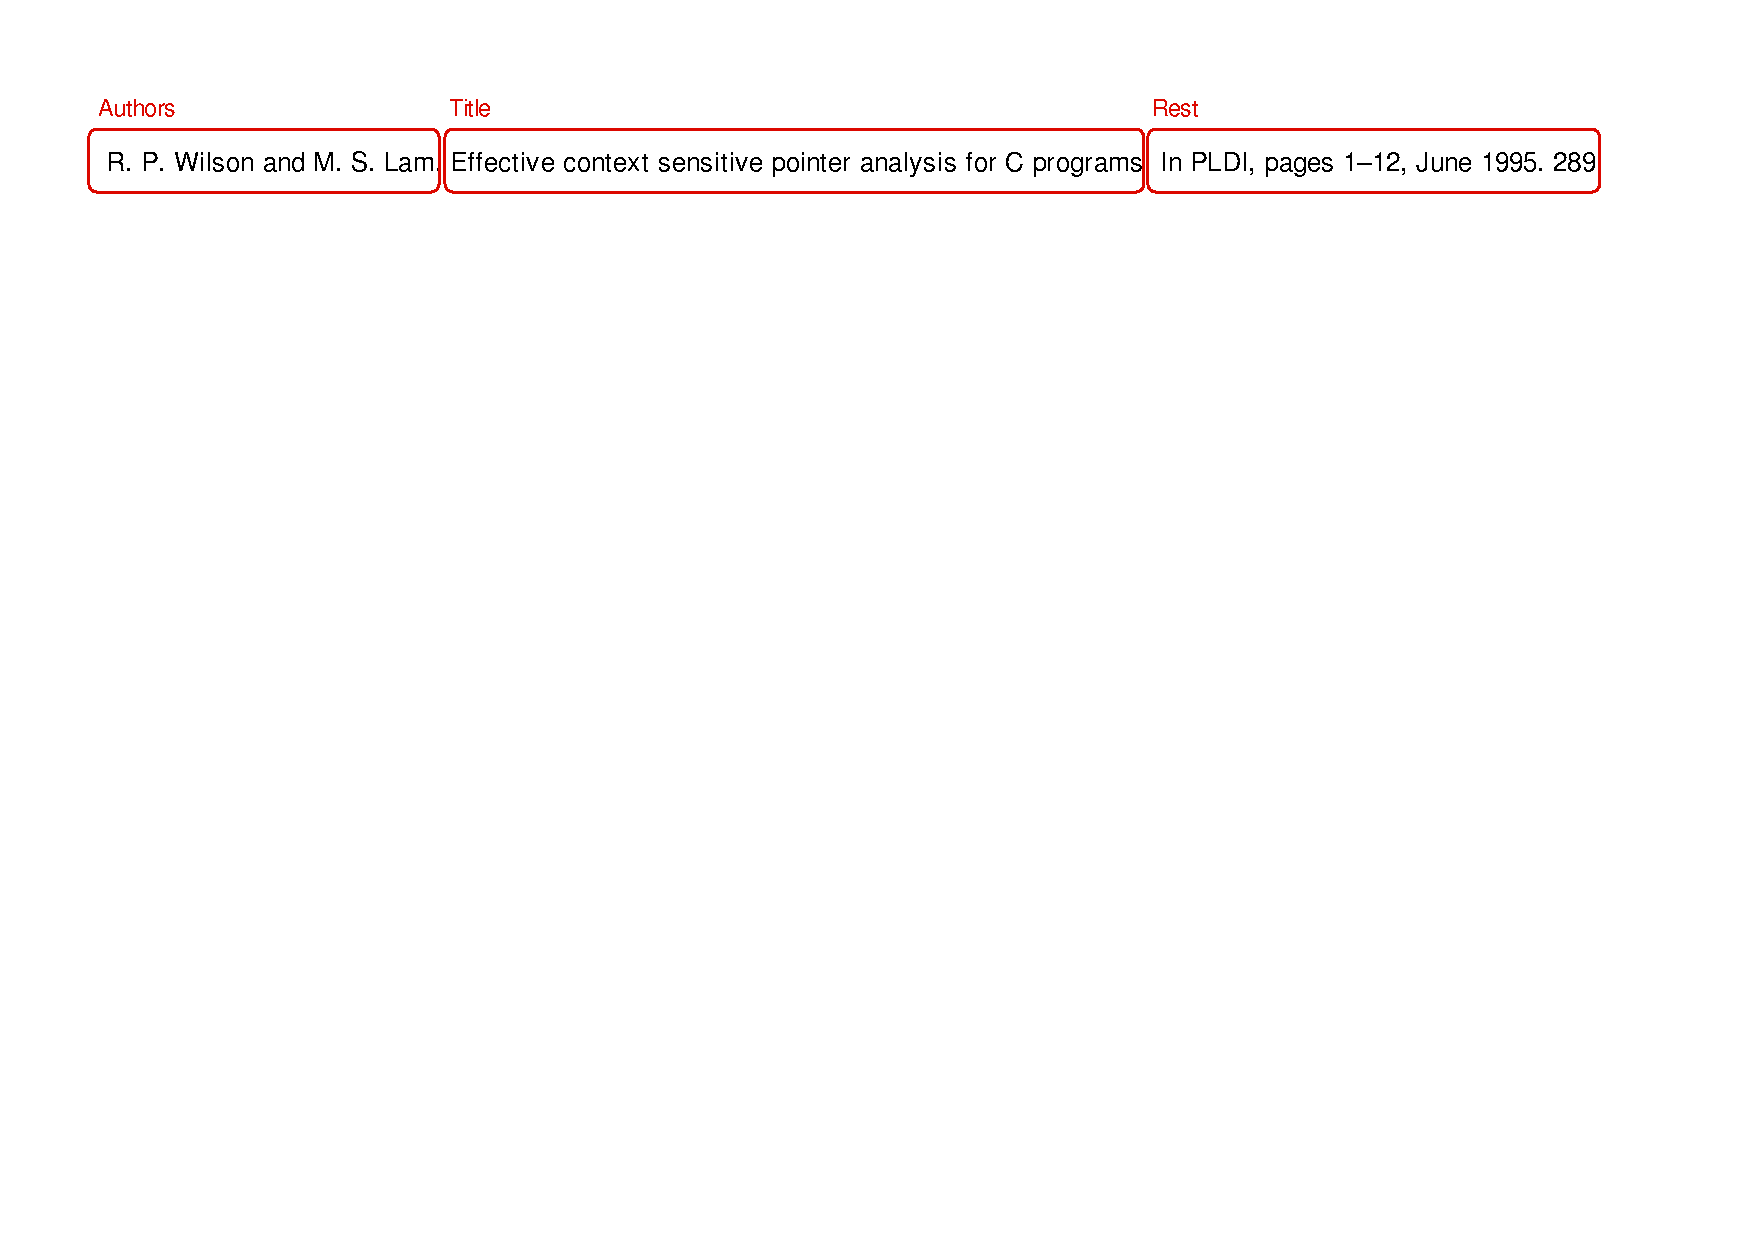
\includegraphics[scale=0.55, trim = 0mm 165mm 0mm 10mm]{link}
    \caption{Common structure of a bibliographic link}
    \label{fig:link}
  \end{figure}     

\subsection{Document Publishing}
There are two systems where documents are published to: Solr and MongoDB. Solr corresponds to a Indexer component and MongoDB corresponds to a Meta Data Storage component in Figure \ref{fig:cs}. We use Solr for indexing citations and MongoDB for storing relations in meta-data. We aim to use MongoDB for aggregating citations referring to the same source paper.

%Solr uses NoSQL-like data storage \brs{this has no meaning. There is a bunch of different NoSQL DBs that are very different from each other, it's like saying ``my file format uses a NoXML like format''} , but actually it is even more limited than traditional NoSQL databases. 
The data stored in Solr is very `flat', which means that Solr cannot store hierarchical data \cite{use.solr1}, \cite{use.solr.2}. In our case, along with the references, we intend to store the title of the scientific article parsed from the reference string, so we can aggregate citations referring to the same scientific article. 
%It should be noted that \ugh{citation itself can refer to multiple scientific articles}\brs{not sure what this means}. 
We are also interested in a solution that does not require reviewing all Solr documents to find citations referring to the same scientific article as it will be too slow and will decrease the quality of the user experience. Thus we use an external storage solution that can keep the titles of scientific articles and all the citations referring to a specific article. As there are few relations in our data and we would like to have a scalable solution we decided to use MongoDB as an external storage.

\paragraph{Publishing documents to Solr}
The common way to interact with Solr is using REST-like API\footnote{\url{http://en.wikipedia.org/wiki/Representational_state_transfer}}. Solr provides client libraries for many programming languages to handle interactions with Solr's REST API. In our project we used SolrJ\footnote{\url{https://cwiki.apache.org/confluence/display/solr/Using+SolrJ}} client library for Java language. This library abstract interaction with Solr into java objects instead of using typical XML request/response format. Basic Solr storage unit is called document and SolrJ has document abstraction implementation. For every detected citation we compose a document to publish. Figure \ref{fig:doc} represents a structure of documents we publish to Solr.

  \begin{figure}[htp]
    \centering
    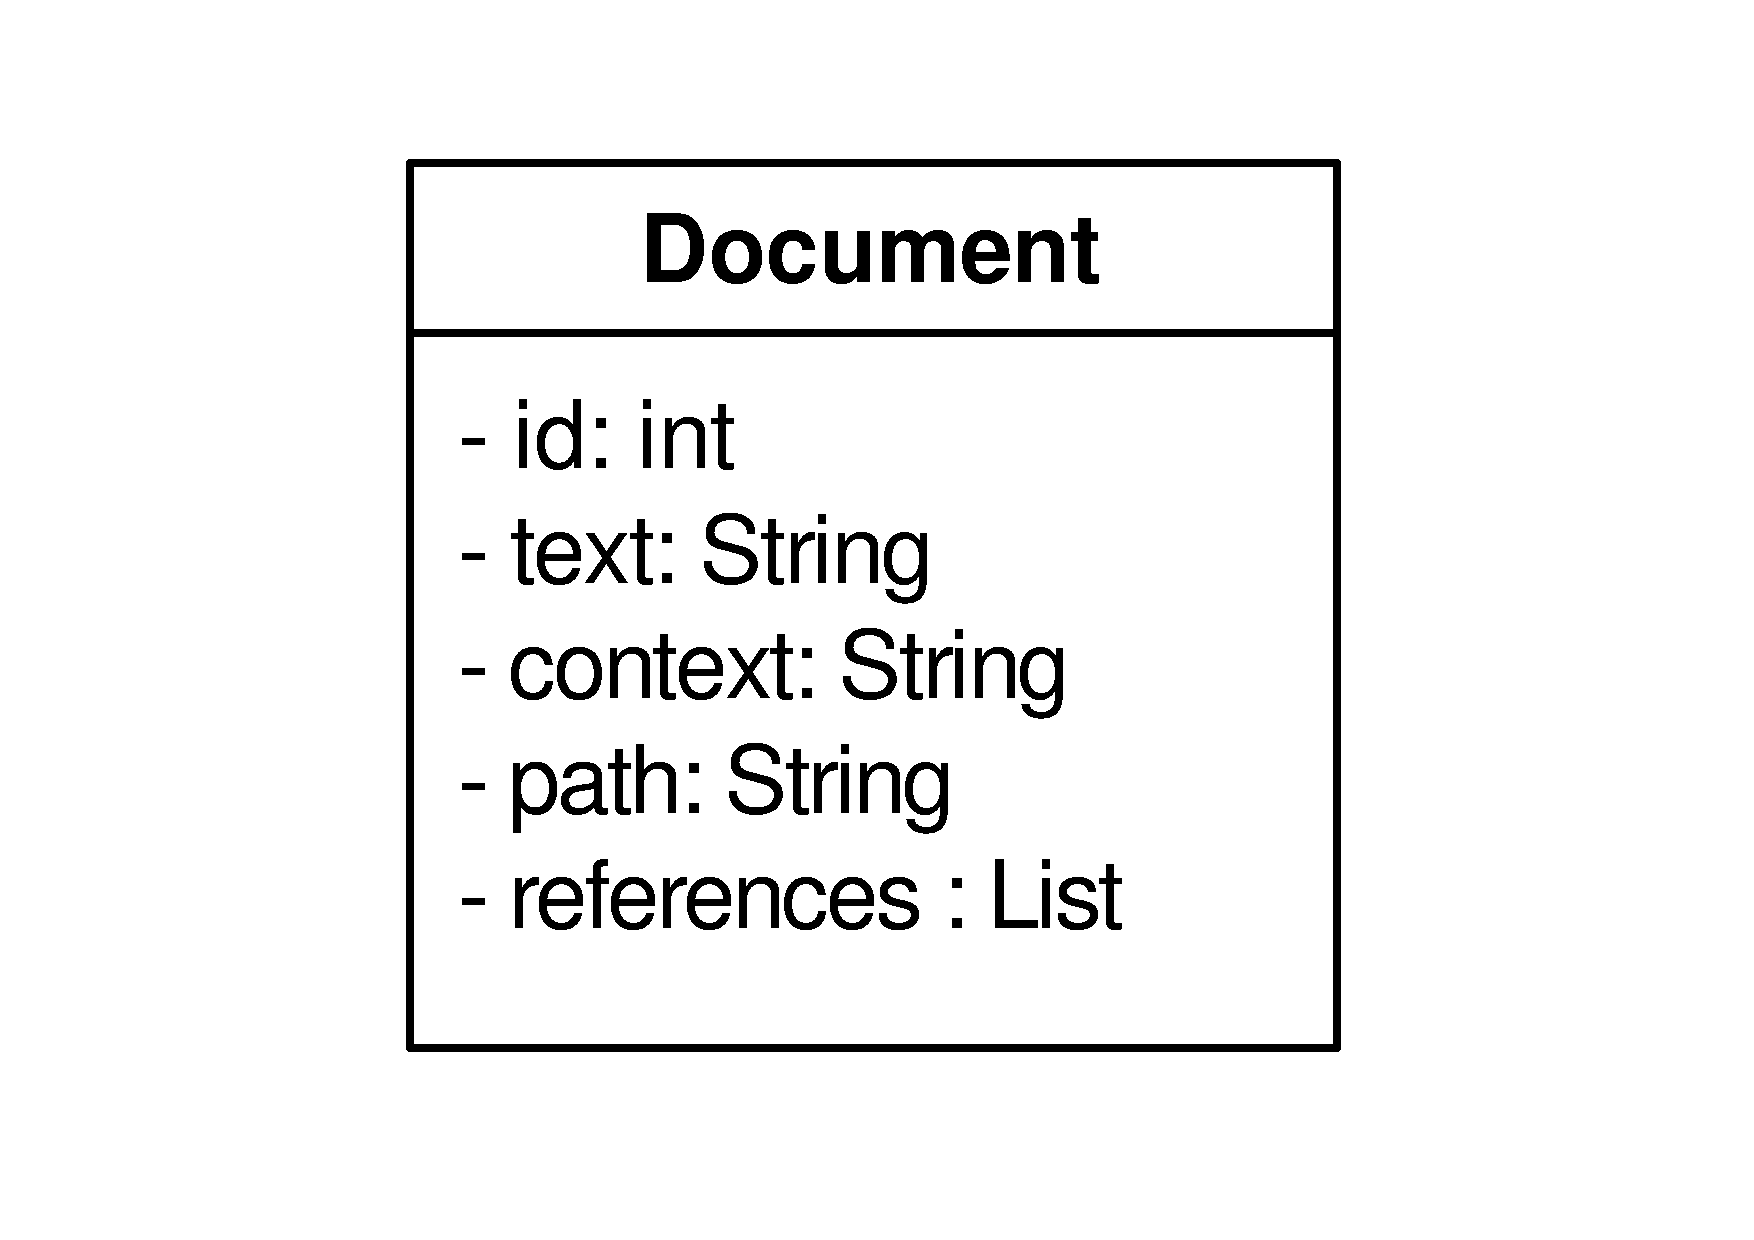
\includegraphics[scale=0.2, trim = 0mm 20mm 0mm 10mm]{doc}
    \caption{Document structure publishing to Solr}
    \label{fig:doc}
  \end{figure} 

Every document representing one citation consist of following fields:
\begin{itemize}[noitemsep]
  \item id: document unique id, mandatory field for publishing to Solr
  \item text: text of the citation that we want to index
  \item context: citation with a text framing it, we take 1 sentence before and 1 after the citation 
  \item path: URL of a document where citation was found
  \item references: list of bibliographic links from references section matching this citation
\end{itemize}

\paragraph{Publishing documents to MongoDB} 
MongoDB is a document-oriented NoSQL database that stores data in JSON-like documents with dynamic schema\footnote{MongoDB database, \url{http://www.mongodb.org/}}. To connect to the database we used a Java driver provided by MongoDB. Although MongoDB is a `schemaless' database we adhere to the JSON structure of the document shown in Listing \ref{lst:json}. 
The json document consist of following fields:
\begin{itemize}[noitemsep]
	\item id: document id, field automatically assigned by MongoDB
	\item title: title of a scientific article
	\item citations: citations with its references of the scientific article identifying by title field 
\end{itemize} 

Every time we send a new citation with a paper title to MongoDB, we check if a document with the same title already exists. If so, we add a new citation to document, otherwise create a new document. \\

\begin{minipage}{\linewidth}
\begin{lstlisting}[label={lst:json}, caption={Sample document stored in MongoDB}]
{ 
	"_id" : ObjectId("547ef1b219795f049d6a0ad0"), 
	"title" : "Re-examining the Fault Density-Component Size  Connection", 
	"citations" : [ 
	{ 
		"citation" : "Hatton, [19], claims that there is “compelling empirical 
					  evidence from disparate sources to suggest that in any 
					  software system, larger components are proportionally more 
					  reliable than smaller components.”", 
		"references" : [ 
		"[19] L. Hatton, “Re-examining the Fault Density-Component Size ..." 
		] 
	}, 
	{ 
		"citation" : "Hatton examined a number of data sets, [15], [18] and 
					  concluded that  there was evidence of “macroscopic behavior” 
					  common to  all data sets despite the massive internal 
					  complexity of each  system studied, [19].", 
		"references" : [ 
		"[15] K.H. Moeller and D. Paulish, “An Empirical Investigation of ...", 
		"[18] T. Keller, “Measurements Role in Providing Error-Free Onboard ...", 
		"[19] L. Hatton, “Re-examining the Fault Density-Component Size  ..." 
		] 
	}] 
}
\end{lstlisting}
\end{minipage}

\section{Indexer}
We use Solr as an Indexer: a solution from Apache Software Foundation built on Apache Lucene. Apache Lucene is an open source, IR library that provides indexing and full text search capabilities\footnote{Apache Lucene, \url{http://lucene.apache.org/core/}}. While web search engines focus on searching content on the Web, Solr is designed to search content on corporate networks of any form. Some of the public service that use Solr as a server are Instagram (photo and video sharing social network), Netflix (movie hosting service) and StubHub.com (public entertainment events ticket reseller). 

Figure \ref{fig:solr} illustrates a high level architecture of Solr. Solr is distributed as a Java web application that runs in any servlet container, for example, Tomcat or Jetty. It provides REST-like web services so external applications can make queries to Solr or index documents. Once the data is uploaded, it goes through text analysis pipeline. In this stage, different preprocessing phases can be applied to remove duplicates in the data or some document-level operations prior to indexing, or to create multiple documents from a single one. Solr comes with a variety of query parser implementations responsible for parsing the queries passed by the end user as search strings. For example, \emph{TermQuery, BooleanQuery, PhraseQuery, PrefixQuery, RangeQuery, MultiTermQuery, FilteredQuery, SpanQuery} and others. Solr has xml configuration files (schema.xml and solrconfig.xml) to define the structure of the index and how fields will be represented and analyzed (see Appendix \ref{app:solr} for Solr installation and configuration).

  \begin{figure}[htp]
    \centering
    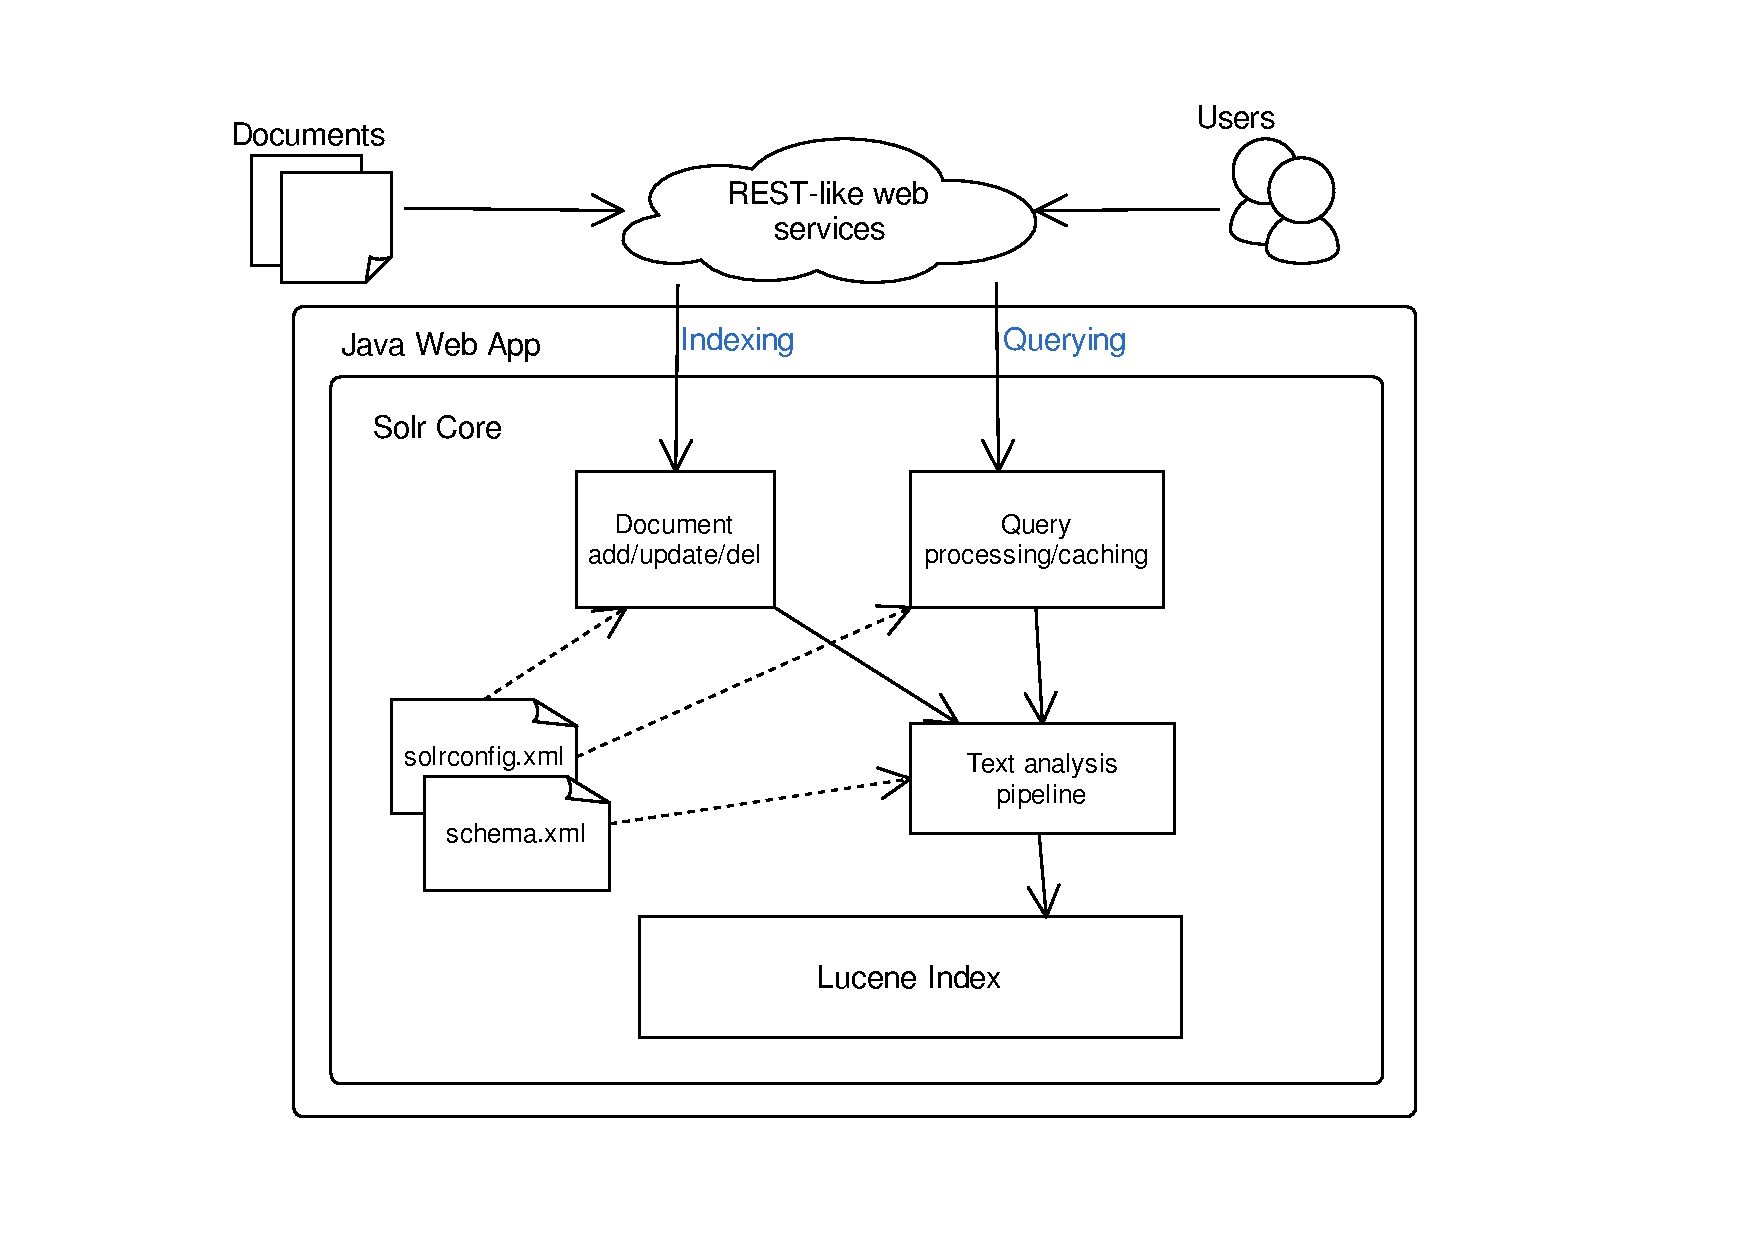
\includegraphics[scale=0.55 , trim = 0mm 10mm 0mm 10mm]{solr}
    \caption{High level architecture of a Solr system}
    \label{fig:solr}
  \end{figure} 

\subsection{Solr Ranking Model}
Solr ranking model is based on the Lucene scoring algorithm, also known as a TF-IDF model \cite{manning2008introduction}. This model takes into consideration following factors:
\begin{itemize}
\item \textbf{tf} - term frequency, a frequency of the term in a document. The higher the term frequency, the higher a document score. 
\item \textbf{idf} - inverse document frequency, an inverse frequency of the term in all documents. The rarer the term occurs in all documents, the higher its contribution to the document's score.  
\item \textbf{coord} - coordination factor, takes into account the number of query terms in a document. The more query terms in a document, the higher score it has. \brs{this is a bit confusing... how does it use query terms to rank? what if it has no queries yet?}
\end{itemize}

The exact scoring formula with the description of all factors can be found on the official web page of the Lucene documentation\footnote{\href{http://lucene.apache.org/java/3_5_0/api/core/org/apache/lucene/search/Similarity.html}{Apache Lucene, scoring formula}}. 

 %\cite{solr.config}

\section{Web Search Interface}
Web Search interface is a Java web application running in a servlet container. Figure \ref{fig:mvc} shows an architecture of a web search application. The application is based on MVC (model-view-controller) architectural pattern implemented with Struts framework\footnote{Struts framework, \url{https://struts.apache.org/}}. The application communicates with Solr via Solr REST API and with Mongo database via Java database connector.  

  \begin{figure}[htp]
    \centering
    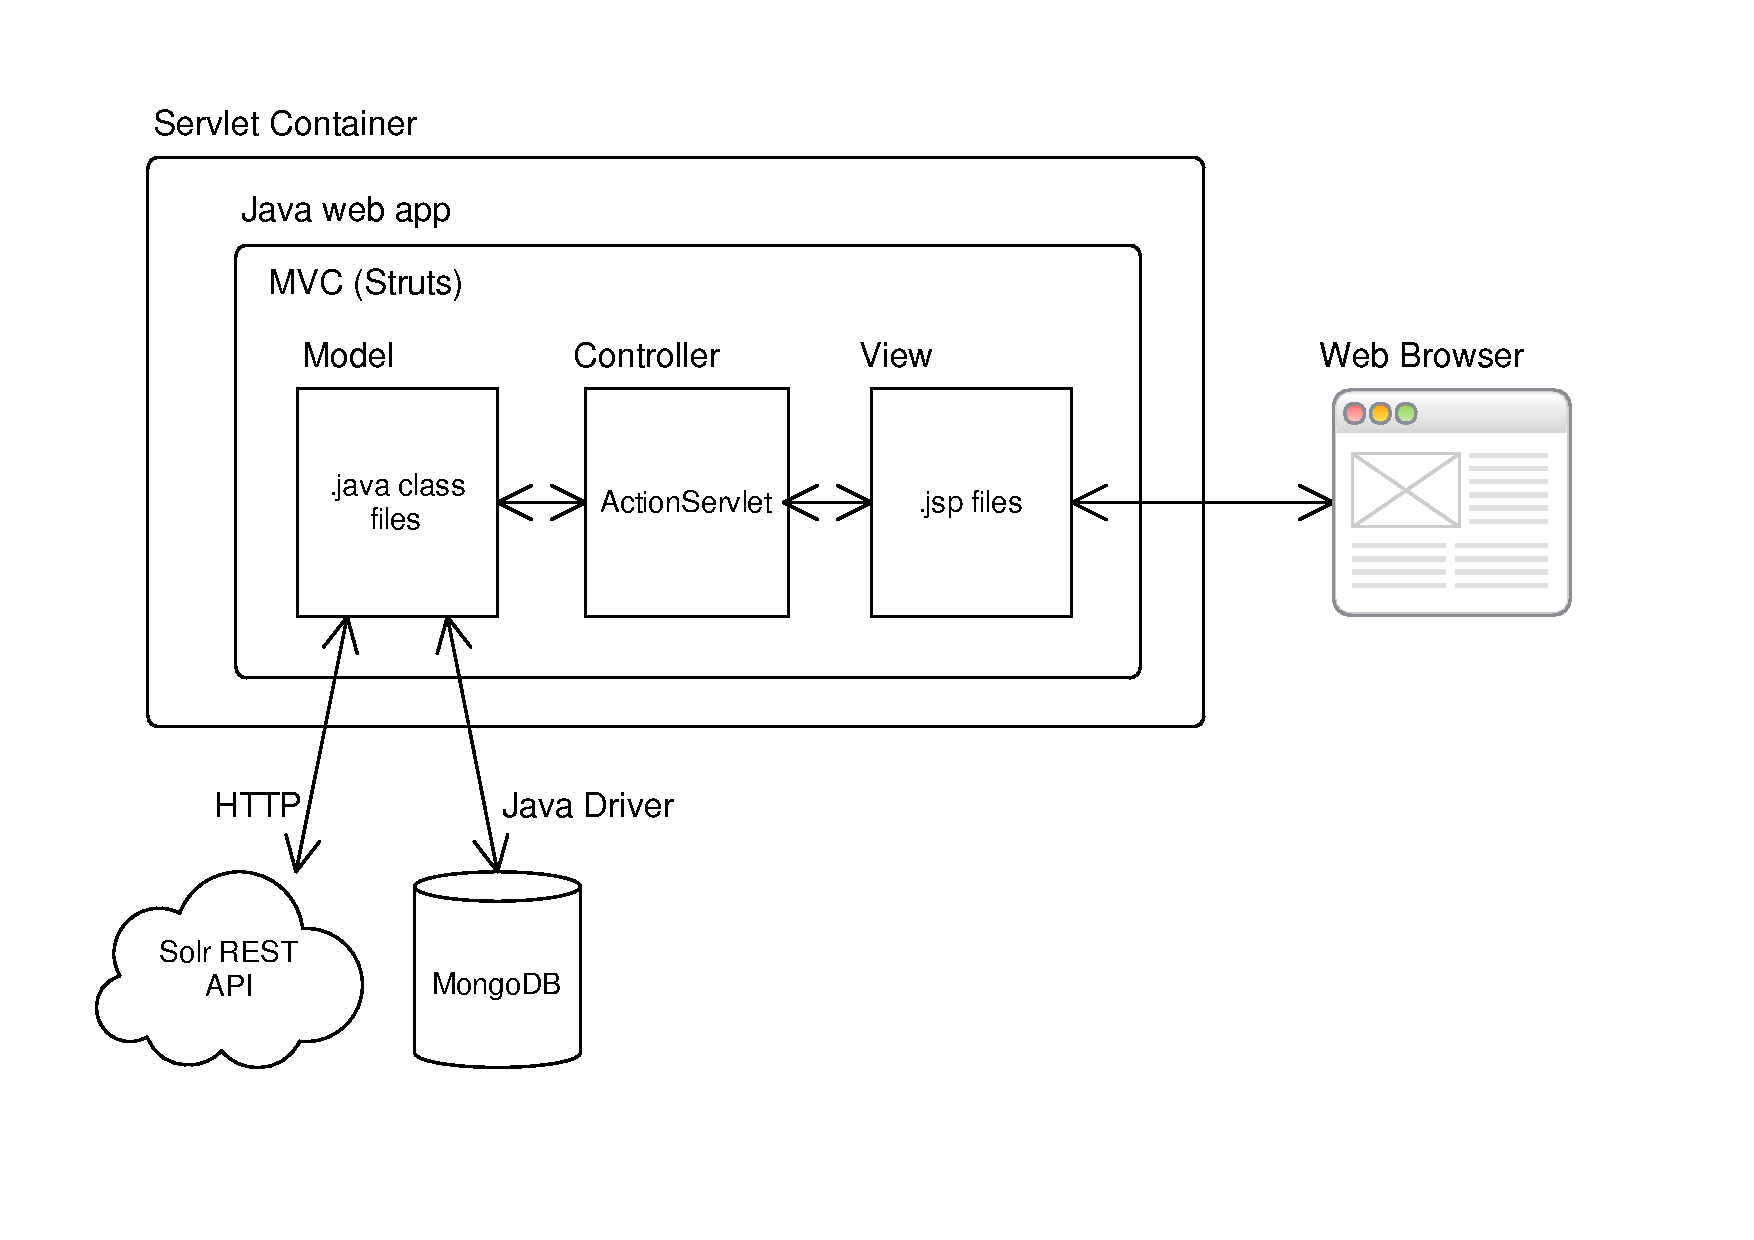
\includegraphics[scale=0.6, trim = 0mm 20mm 0mm 10mm]{struts}
    \caption{Architecture overview of a web search application}
    \label{fig:mvc}
  \end{figure}  

\subsection{CiteWise Main Page}

The main page of CiteWise presents a simple search interface allowing user to search for citations. Figure \ref{fig:cs-main-page} shows a sample response to the user query ``software testing is time-consuming''. As a result a user sees a list of documents matching the query. Each document has a citation with a list of bibliographic links supporting this citation. A user can click to ``Show context'' link to see a text surrounding the citation in the original paper. If the source paper is available then user can open it using a link ``See pdf on SCG resources''.  

  \begin{figure}[htp]
    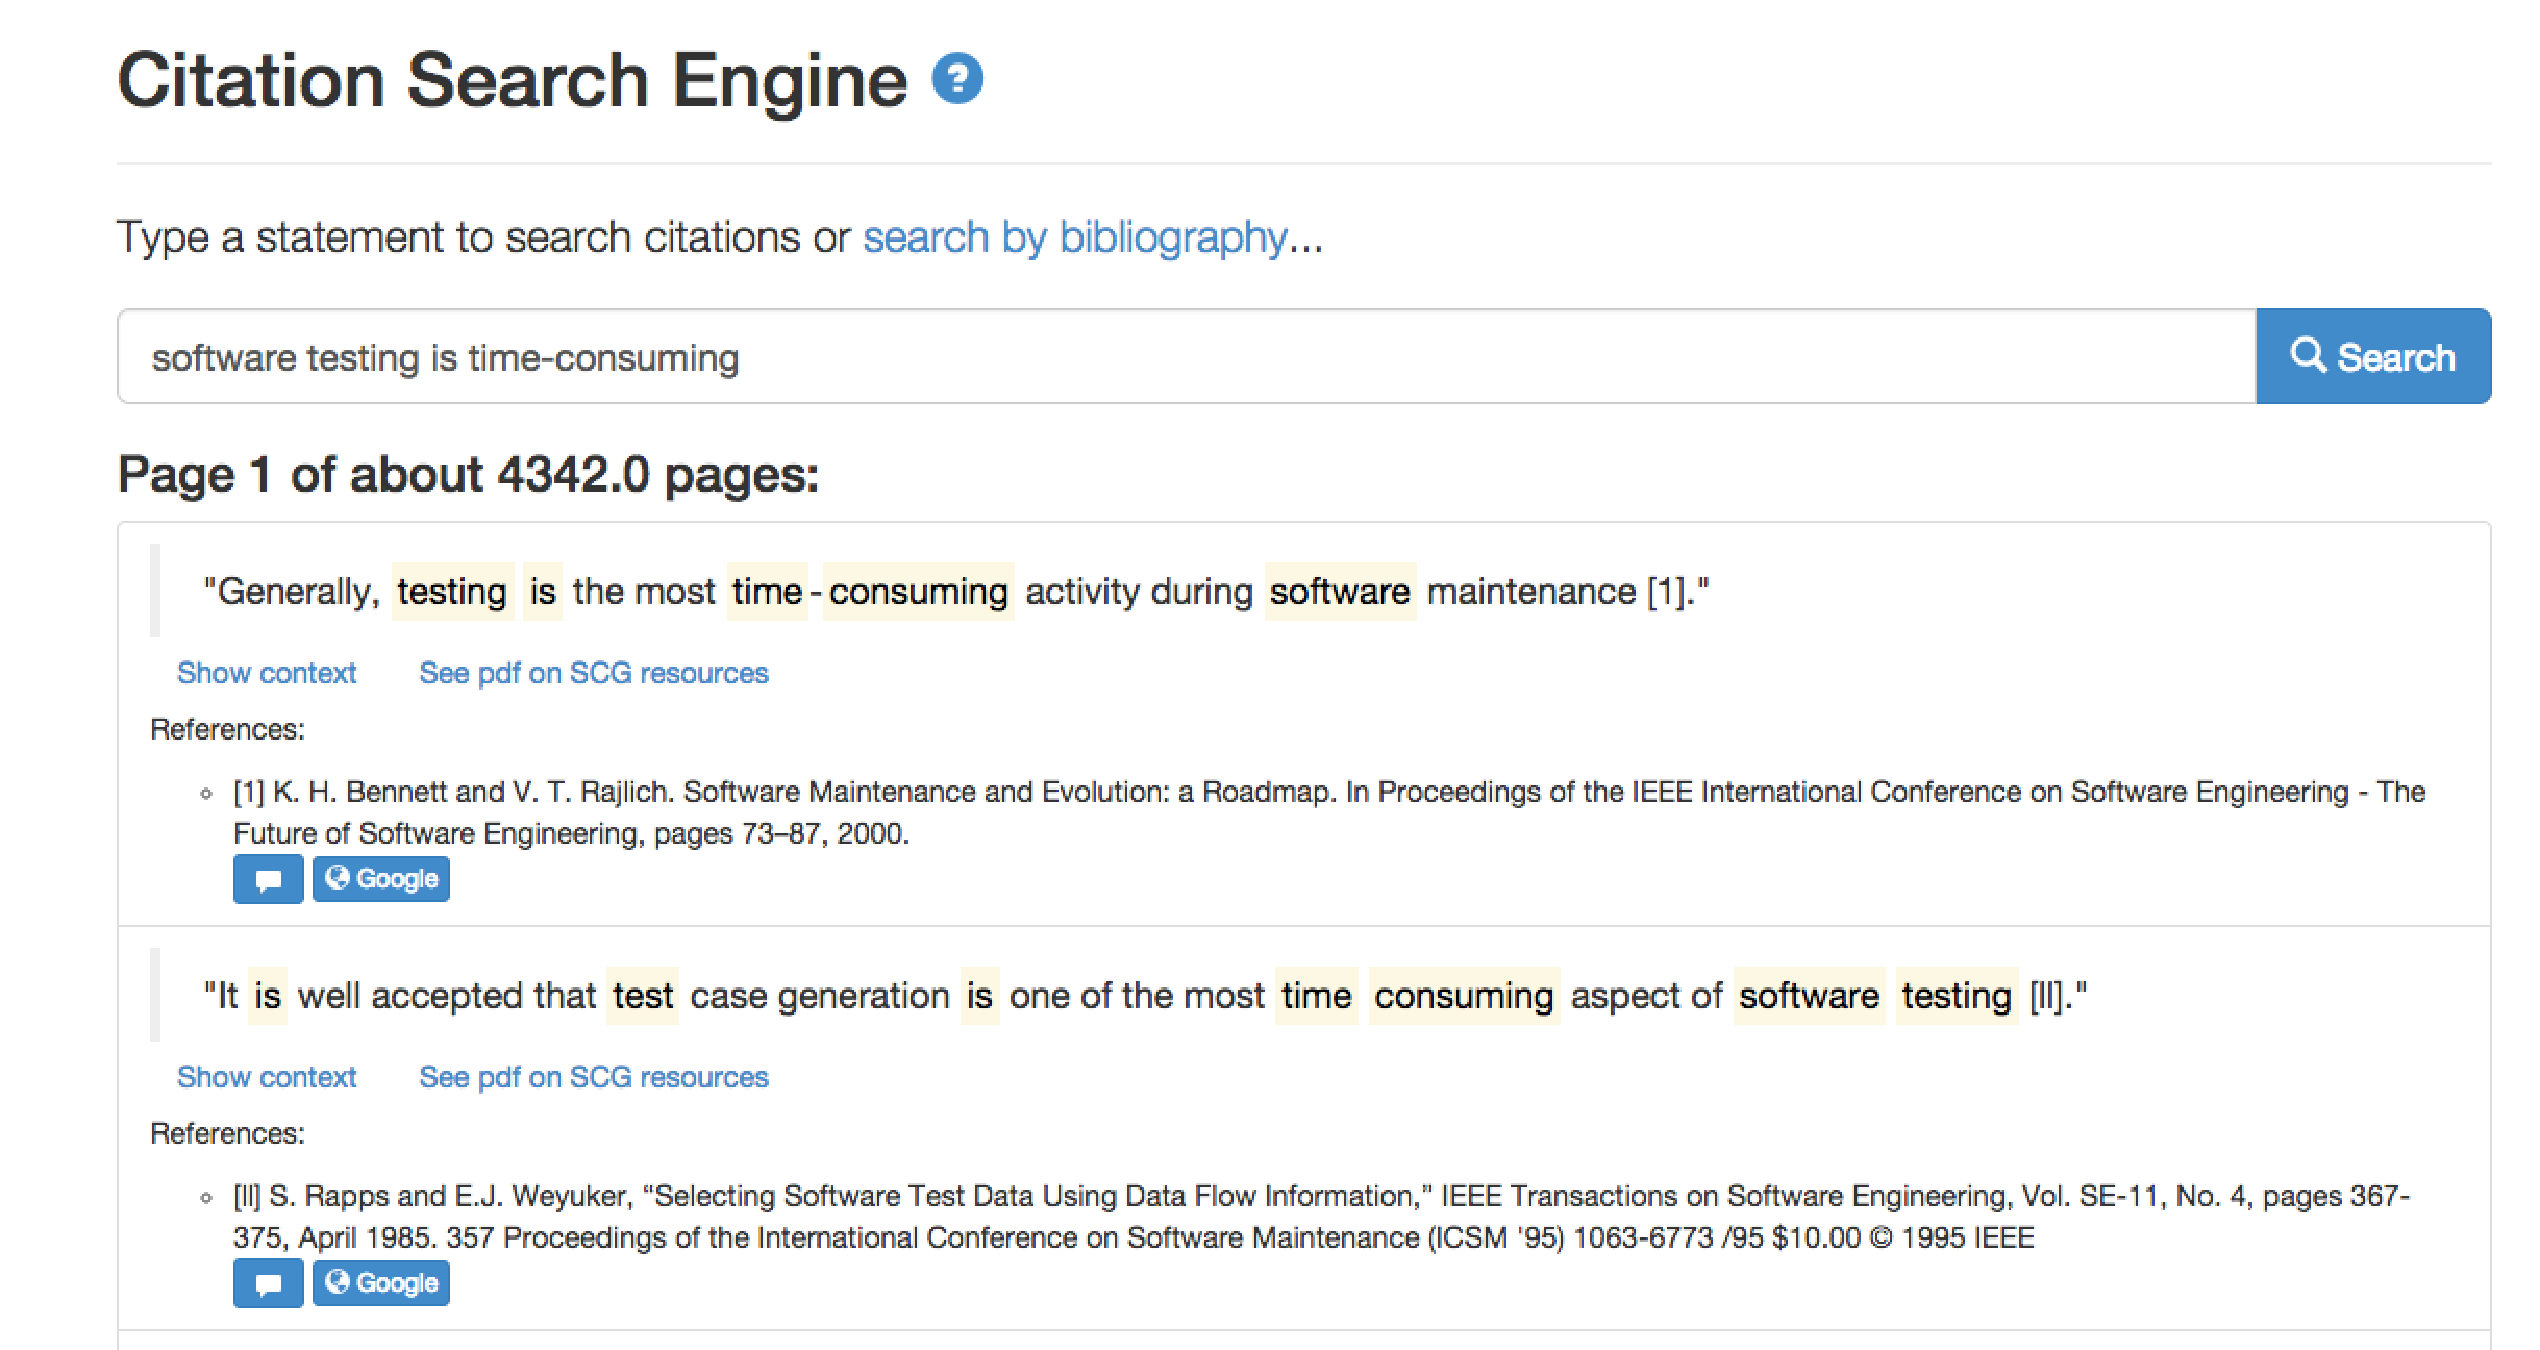
\includegraphics[scale=0.4, trim = 0mm 0mm 0mm 0mm]{cs-main-page}
    \caption{A screenshot of the main page of the CiteWise interface showing results for a statement query ``software testing is time-consuming''}
    \label{fig:cs-main-page}
  \end{figure}

If a reference has a title recognizable by CiteWise then a user can see all citations referring to the paper from this reference by clicking on the button next to the reference. Figure \ref{fig:cs-view-citations} demonstrates this feature. A user can see all citations of the paper ``Software maintenance and evolution: a roadmap'' in a popover dialog. User can get more information on each citation by following a ``View details'' link.

   \begin{figure}[htp]
    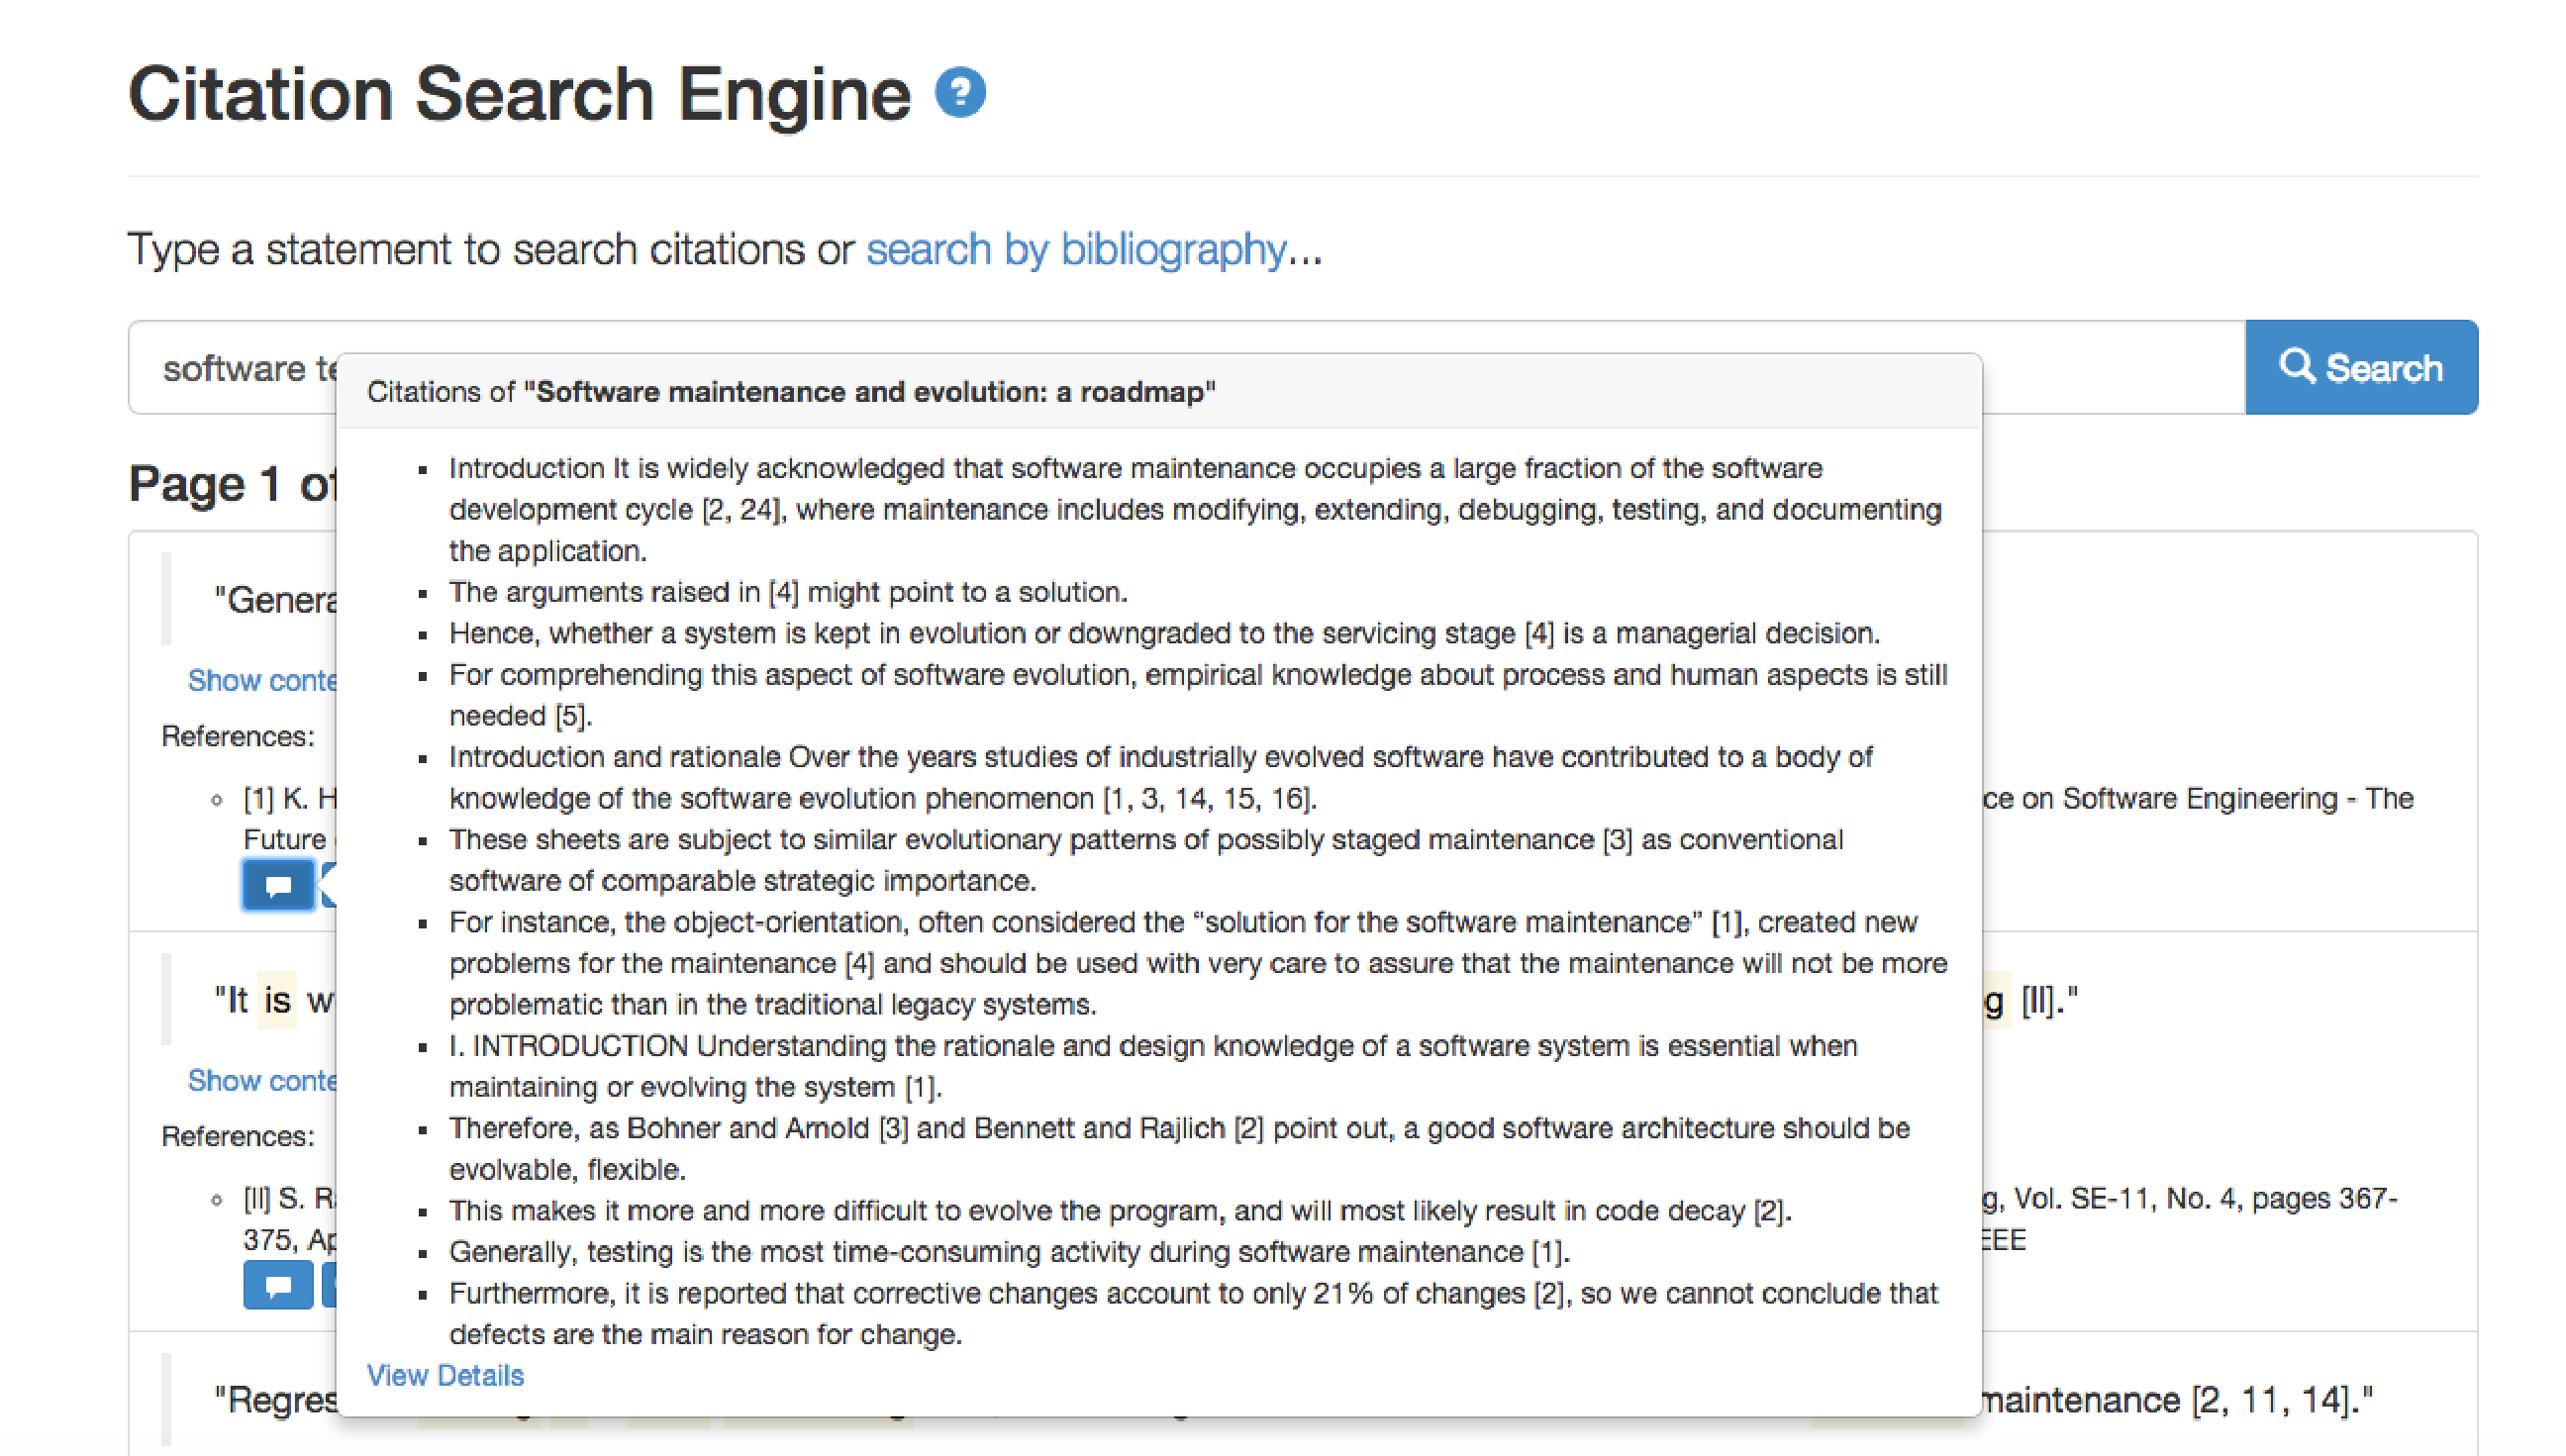
\includegraphics[scale=0.4, trim = 0mm 0mm 0mm 0mm]{cs-view-citations}
    \caption{A screenshot of the main page of a CiteWise interface showing citations referring to the article with the recognizable title ``Software maintenance and evolution: a roadmap.''}
    \label{fig:cs-view-citations}
  \end{figure}

A user can take advantage of using enhanced search query syntax. The query syntax is explained on the help page of the CiteWise interface and in the Appendix of this article.

\subsection{Search by Bibliography Page}
Another feature provided by CiteWise is the possibility to search by bibliography entries. For example, a user can search by authors, title or publication venue. An example of a search by author is shown in Figure \ref{fig:cs-search-bibl}. A user sees a list of bibliographic entries with searched author name. If an entry has an extractable title then user can see citations from other papers referring to the entry.

   \begin{figure}[htp]
    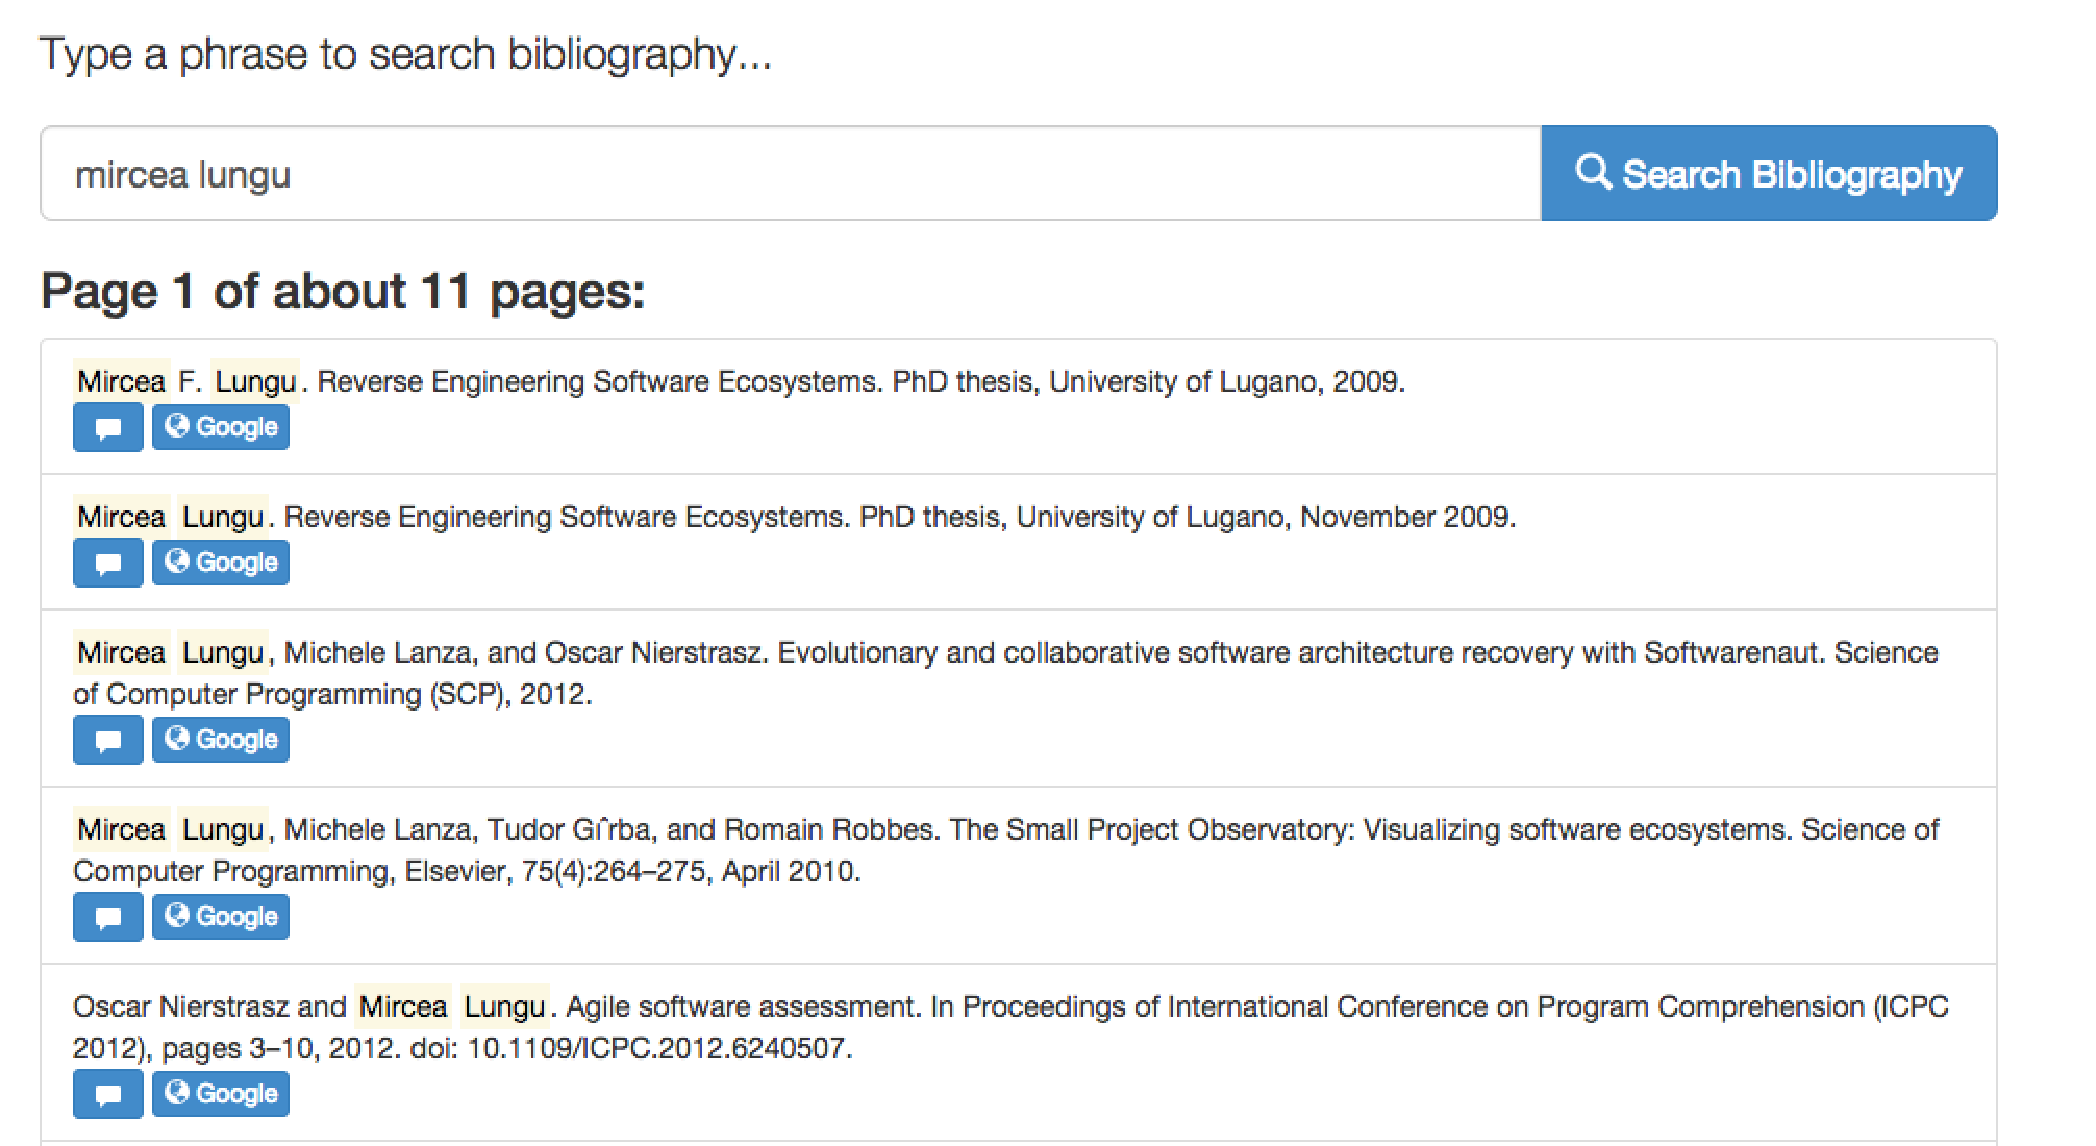
\includegraphics[scale=0.4]{cs-search-bibl}
    \caption{A screenshot of the `search by bibliography' page of a CiteWise interface illustrating a search for citations based on a meta-information query. Here a user searches for citations of scientific articles authored by Mircea Lungu.}
    \label{fig:cs-search-bibl}
  \end{figure}

\chapter {Evaluation}
\label{cha:experiments}
To measure the effectiveness of CiteWise we conducted evaluation experiments comparing it with other search engines.  We had two main candidates to compare CiteWise with: CiteSeerX and Google Scholar.

Preparatory tests showed that CiteSeerX is too slow in showing results. Moreover, users complained that resulting documents are not relevant. Too many results were from a different domain than Computer Science, like Biology or Physics.  Thus, all experiments were conducted with Google Scholar and CiteWise. 

There are many aspects on how two search engines might be compared. In our experiments we focused on efficiency and usability. By efficiency we imply how quickly users can find documents and by usability we imply simplicity of search interfaces and personal impression.

\section{Experiment Setup}
\subsection{Data and Tools}
For evaluation experiments we used a dataset of scientific articles collected by SCG\footnote{\url{http://scgresources.unibe.ch/Literature/}} members over decades. The collection contains about 16000 scientific articles and covers various topics in Software Engineering and Programming Languages. The Google Scholar dataset is much larger that the data set used in our experiments, so we reduced the searching space to the domain of Software Engineering and Programming Languages. During the experiment all participants were provided with a laptop (MacBook Air, OS X version 10.10.3) and their actions were recorded with a screen casting application (QuickTime Player).

\subsection{Participants}
We intentionally looked for experts in the domain of Software Engineering and Programming Languages that can participate in experiments. Nine experts with different experiences (7 PhD candidates, 1 postdoctoral researcher, 1 professor) participated in experiments ( see Table \ref{tab:experts}).
\begin{table}[ht]
\begin{center}
\begin{tabular}{  c | c | c | c } 
 \hline
 \textbf{ID} & \textbf{Position} & \textbf{Domains of Interest} &\textbf{Years} \\ \hline
 P1 & Professor researcher & Software Engineering and Programming Languages & 35\\
 P2 & PostDoc researcher & Software and Ecosystem Analysis & 11  \\ 
 P3 & PhD candidate & Software Quality & 2 \\   
 P4 & PhD candidate & Ecosystem Analysis & 2 \\
 P5 & PhD candidate & Dynamic Analysis & 2 \\  
 P6 & PhD candidate & Software Architecture & 3 \\
 P7 & PhD candidate & Development Tools & 3 \\
 P8 & PhD candidate & Parsing & 3 \\ 
 P9 & PhD candidate & Software Visualization & 1 \\ 
 \hline  
\end{tabular}
\caption{The table describes experts which participated in the experiments, their domain of interests and academic experience in years.}
\label{tab:experts}
\end{center}
\end{table}


\subsection{Process}
Participants were split into two groups. All experiments were conducted in two days and each day was dedicated to one group. Both groups were asked to perform the same tasks. However the second group was asked to do one more additional task (see Table \ref{tab:groups}). The idea of giving an additional task to the second group came after conducting experiments with the first group on the first day. Time given to complete each task was limited to 5 minutes. All tasks are described in subsection Tasks \ref{sub:tasks}.  
\begin{table}[ht]
\begin{center}
\begin{tabular}{  c | c | c  } 
 \hline
 \textbf{Groups} & \textbf{Participants} & \textbf{Tasks to perform} \\ \hline
 Group1 & P1, P3, P4, P5, P6 & Task 1a, Task 2\\
 Group2 & P2, P7, P8, P9 & Task 1a, Task 1b, Task 2\\  
 \hline  
\end{tabular}
\caption{Devision of participants by groups and tasks given to each group.}
\label{tab:groups}
\end{center}
\end{table}

Each experiment was setup to last for approximately 45 minutes and each experiment involved only one participant. An experiment starts with a short training session, where we introduce the participant to: 1) user interfaces of both CiteWise and Google Scholar, 2) standard syntax query common to both search engines. Every task in the experiment was orally explained to the participant.

\subsection{Tasks}
\label{sub:tasks}
\paragraph{Task 1a} As a first task, a participant was asked to find a reference to a claim from one of his papers written in the past using CiteWise or Google Scholar. We specified the type of the search engine in the beginning of the task. A test subject can read the cited sentence as well as the context of this sentence but is not aware of the referred source paper. The task is to find a paper that proves the given citation. We use following procedure to conduct Task 1a:
\\Before the experiment.
\begin{enumerate}
	\item We look for a paper published by the test subject.
	\item We extract four citations from that paper.
	\item We delete extracted citations from CiteWise so the test subject could not find an exact match using CiteWise.
\end{enumerate}
During the experiment.
\begin{enumerate}
	\item We let the test subject read one cited sentence as well as the context of this sentence.
	\item We ask the test subject to find a referred paper that proves the given claim using the given search engine (CiteWise or Google Scholar).
	\item We repeat steps for four citations every time changing the used search engine. 
\end{enumerate}
\brs{make clear what the chose if search engine is! does the subject chose the first time and then it alternates? if not which was the first one? etc.}

During the execution of tasks, we observe the following:
\begin{itemize}[noitemsep]
	\item \emph{Search time}, time spent by participant to find a paper supporting the given cited text. 
	\item \emph{Number of queries}, the amount of queries made by participant to find a reference.
	\item \emph{Number of words in each query}, numbers of words in each query made by the test subject while searching.
	\item \emph{Expert comments}, any comments made by the test subject during the task execution.
\end{itemize}  

\paragraph{Task 1b} Task 1b was given to the second group as an extra task. By conducting this task, we would like to know which search engine would the test subject use if it is not specified in the task description. As in Task 1a a test subject was also given a citation to find a reference to, but this time a search engine was not specified and a citation was taken from a paper not authored by test subject. Every participant received only one citation for this task. As for the previous task the citation was removed from CiteWise before the experiment. 

During Task 1b, we observed which search engine was used to find a reference. 

\paragraph{Task 2} In Task 2 we asked participants to compare two summaries generated with CiteWise and TextRank\cite{mihalcea2004textrank} algorithms\brs{this was not mentioned in the beginning of the evaluation section, you said all experiments where conducted with Google Scholar}. The TextRank algorithm is a graph-based ranking algorithm for Natural Language Processing (NLP) \cite{mihalcea2004graph}. It extracts sentences from the text based on their importance. We use following procedure to conduct Task 2:
\\Before the experiment.
\begin{enumerate}
	\item We ask every participant in advance to provide a paper that she thinks is important in her research field. 
	\item We verify that a provided paper was cited at least by ten other papers in the CiteWise dataset.
	\item We build a first summary using the TextRank algorithm. We use a Python implementation of this algorithm that can be found on GitHub \footnote{\url{https://github.com/adamfabish/Reduction}}. We extract the text of a paper and feed it to TextRank. We limit the size of summaries to the size of an abstract in a paper, that is approximately 9-10 sentences.
	\item We build a second summary using citations to the paper collected by CiteWise. CiteWise might collect more than ten citations of a paper. In this case we pick ten sentences randomly. Again we limit the size of summaries to the size of an abstract in a paper. 
\end{enumerate}
During the experiment.
\begin{enumerate}
	\item We let the test subject read two summaries.
	\item We ask test subjects to access quality of summaries by giving a score from 0 to 10.
\end{enumerate}

\section{Questionnaires}

\subsection{Pre-experiment Questionnaire}
Before the beginning of the experiment we ask the test subjects to provide preliminary information by filling in a pre-experiment questionnaire. The goal of the pre-experiment questionnaire is to gather general statistics about the participants' experience in using various search engines. We ask the participants to fill in a form with following questions:
\begin{itemize}
	\item What search engines do you usually use to find scientific literature?
	\item How often do you use the listed search engines? (Possible answers: everyday, a few times per week, once a week or less)
	\item Have you ever used the following search engines?(Google Scholar, CiteWise )
\end{itemize} 

\subsection{Debriefing interview}
After completing Task 1a and Task 1b we conduct a semi-structured interview with participants, that lasts approximately 5 minutes. The main goal of the debriefing interview is to get an immediate feedback on using Google Scholar and CiteWise. During the interview the participants have chance to share their impression on using both search engines. Sample questions asked during the interview:
\begin{itemize}
	\item What did you like/dislike about using each search engine?
	\item What difficulties did you have?
\end{itemize}

\subsection{Post-experiment Questionnaire}
Right after the experiment we ask the participant to fill in a post-experiment questionnaire. The main goal of the post-experiment questionnaire is to gather further feedback on using CiteWise and Google Scholar. We ask the participants to fill in a form with following questions:
\begin{itemize}
	\item Has the experiments changed your opinion on the two search engines?
	\item Would you consider using one of these search engines? 
\end{itemize}

\section{Evaluation Results}

The pre-experiment questionnaire showed that almost all participants (8 experts) use Google Scholar to find scientific literature. Some participants mentioned that they use IEEE Explorer, ACM digital library and DBLP as well (see Table \ref{tab:q1_1}). Half of the respondents (4 participants) use search engines daily, 2 respondents use search engines a few times per week (see Table \ref{tab:q1_2}).

\begin{table}[ht]
\begin{center}
\begin{tabular}{  c | c | c | c | c  } 
 \hline
 \textbf{Participants} & \textbf{Google Scholar} & \textbf{DBLP} & \textbf{IEEE Xplore} & \textbf{ACM Library} \\ \hline
 P1 & \checkmark & \checkmark & & \\
 P2 & \checkmark & \checkmark & & \\
 P3 & \checkmark & & \checkmark & \checkmark \\ 
 P4 & \checkmark & & & \\ 
 P5 & \checkmark & & & \\  
 P6 & \checkmark & & & \\ 
 P7 & & & \checkmark & \checkmark\\
 P8 & \checkmark & & & \\
 P9 & \checkmark & & & \\   
 \hline 
 \textbf{Total} & 8 & 2 & 2 & 2\\  
\end{tabular}
\caption{Pre-Experiment Questionnaire. The table shows total number of participants using particular search engine to find scientific literature.}
\label{tab:q1_1}
\end{center}
\end{table}

\begin{table}[ht]
\begin{center}
\begin{tabular}{  c | c | c | c } 
 \hline
 \textbf{Participants} & \textbf{Every day} & \textbf{A few times per week} & \textbf{Once a week or less} \\ \hline
 P1 & \checkmark & & \\
 P2 & & \checkmark & \\
 P3 & \checkmark & & \\ 
 P4 & & &\checkmark \\ 
 P5 & \checkmark & & \\  
 P6 & & &\checkmark\\ 
 P7 & & \checkmark &\\
 P8 & & & \checkmark \\
 P9 & \checkmark & & \\   
 \hline 
 \textbf{Total} & 4 & 2 & 3\\  
\end{tabular}
\caption{Pre-Experiment Questionnaire. The table shows how often participants use search engines to find scientific literature. }
\label{tab:q1_2}
\end{center}
\end{table}

Four respondents answered positively on the question if they have ever used CiteWise. However all of them mentioned that they used CiteWise only a few times.

\subsection{Results for Task 1a}  
In Task 1a we measured search time. Each participant perofrmed Task 1a 4 times: 2 times with CiteWise and 2 times with Google Schoalr. In overall, we made 18 measurements for CiteWise and 18 measurements for google Schoalr. Figure \ref{fig:boxplot-search-time} illustrates results for search time in Task 1a using boxplots \footnote{\url{http://en.wikipedia.org/wiki/Box_plot}}. Table \ref{tab:search-time} shows the mean and standard deviation of search times for both search engines. From Table \ref{tab:search-time} we observed that the average time to find a reference for a given citation is approximately 2.5 minutes. Participants were slightly faster with finding results using CiteWise. However, there is no statistically significant difference between search times of CiteWise and Google Scholar according to t-test with significance level p = 5\%. 

  \begin{figure}[htp]
    \centering
    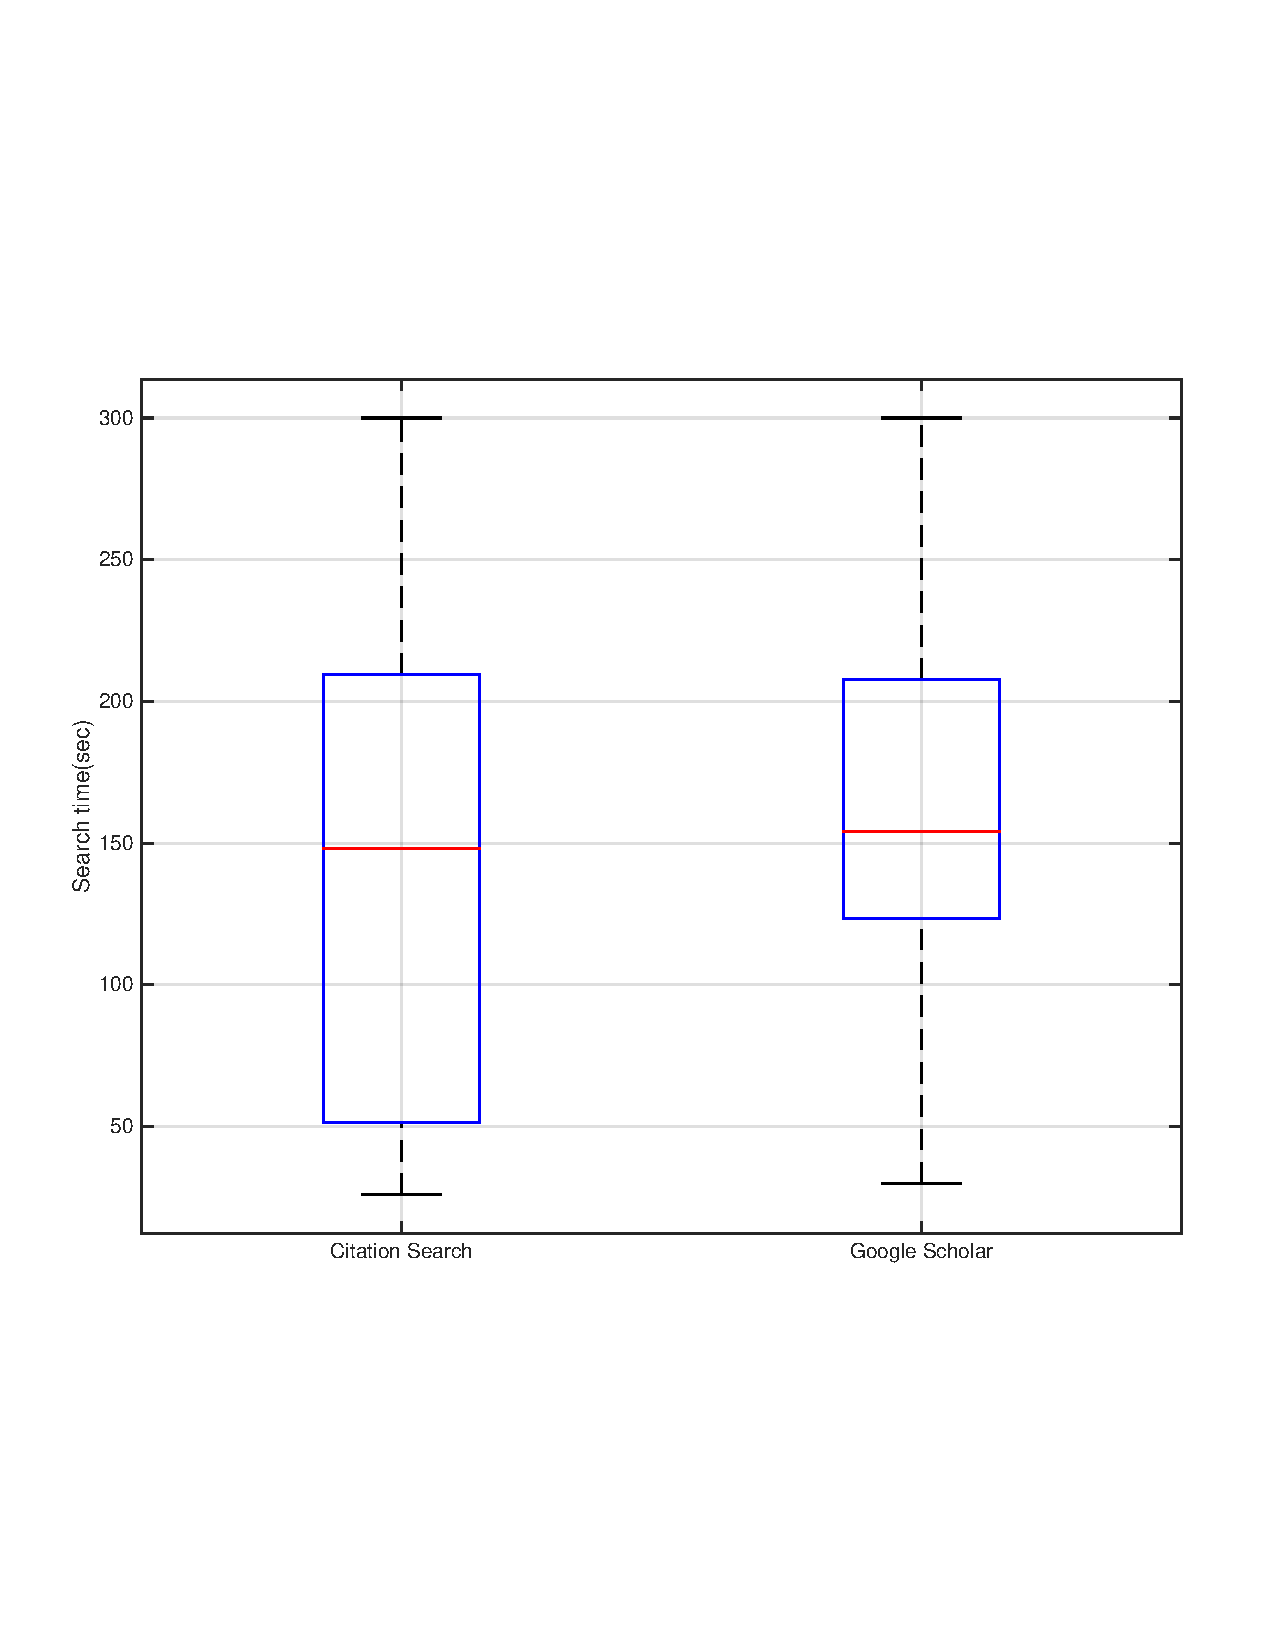
\includegraphics[scale=0.6, trim = 0mm 60mm 0mm 50mm,]{boxplot-search-time}
    \caption{Boxplot of search times in Task 1a for both search engines. The red band inside a box is a second quartile (the median). The bottom and top of the box are the first and third quartiles. The end of whiskers represent the minimum and maximum values for search times. \brs{mark the axis on the plot}}
    \label{fig:boxplot-search-time}
  \end{figure}

\begin{table}[ht]
\begin{center}
\begin{tabular}{ | c | c | c | } 
 \hline
 & \textbf{Mean(sec)} & \textbf{Std(sec)} \\  \hline
 CiteWise & 150 & 97\\ \hline
 Google Scholar & 160 & 78  \\    
 \hline
\end{tabular}
\caption{The mean and standard deviation of search times for CiteWise and Google Scholar in Task 1a.}
\label{tab:search-time}
\end{center}
\end{table}

Table \ref{tab:search-query} shows average values and standard deviations for number of queries made by experts to find references and average number of words in queries. We did not see any significant differences in a number of queries and average number of words in a query between two search engines. From Table \ref{tab:search-query} we concluded that in average participants made 2-3 queries before finding a referred paper and that the average number of words in a query was 4.

 \begin{table}[ht]
\begin{center}
\begin{tabular}{  c | c | c  } 
 \hline
 & \textbf{Mean} & \textbf{Std} \\  \hline
 \textbf{Number of queries} & & \\ \hline
 CiteWise & 2.0 & 1.5\\ 
 Google Scholar & 2.5 & 1.5  \\  \hline 
 \textbf{Average number of words in a query} & & \\ \hline 
 CiteWise & 4.3 & 1.7\\
 Google Scholar & 4.2 & 1.2  \\     
 \hline
\end{tabular}
\caption{The mean and standard deviation values for a number of queries and avearge number of words in a query in Task 1.}
\label{tab:search-query}
\end{center}
\end{table}

 During the experiments we noticed that participants were more familiar with Google Scholar search interface so participants spent some time exploring CiteWise interface. This could affect search time for CiteWise making it longer.

We also noted that the way search engines present results is an important factor of the search engine usability. For example, most of the participants admitted that they like that CiteWise shows the exact place from the article where match was found. In contrast, Google Scholar shows a title of the article and a beginning of the abstract, so it is not clear where the match was found. In this case participants had to open the article and make a manual search over the text.  

\subsection{Results for Task 1b}
Task 1b was given to four participants. Table \ref{tab:se-any} shows in what search engine a referred paper was found and if a participant tried to use both search engines. From Table \ref{tab:se-any} we concluded that all participants found a referred paper using CiteWise. Meantime three of participants tried both search engines and one participant did not use Google Scholar at all. 

\begin{table}[ht]
\begin{center}
\begin{tabular}{ c | l } 
 \hline
 \textbf{Participants} & \textbf{How search engines were used} \\  \hline
 P6 & CiteWise, Google Scholar, \textcolor{red}{CiteWise} \\ \hline
 P7 & Google Scholar, \textcolor{red}{CiteWise}  \\ \hline
 P8 & Google Scholar, \textcolor{red}{CiteWise}  \\ \hline
 P9 & \textcolor{red}{CiteWise} \\   
 \hline
\end{tabular}
\caption{Results for Task 1b. The table shows in what search engine a result was retrieved and if a participant tried to used both search engines during the task.}
\label{tab:se-any}
\end{center}
\end{table}  

\subsection{Results for Task 2}

Results for Task 2 are shown in Figure \ref{fig:summaries}. It illustrates scores from 0 to 10 given by participants to summaries generated with TextRank and citation from CiteWise.  
  \begin{figure}[htp]
    \centering
    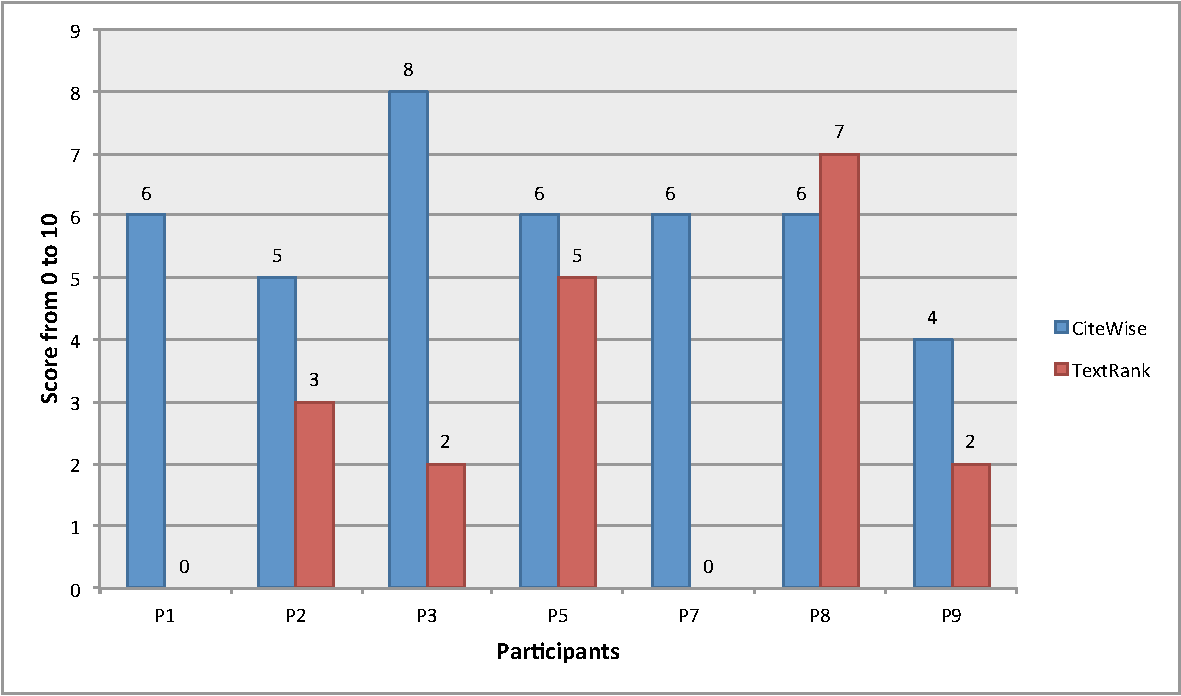
\includegraphics[scale=0.7, trim = 0mm 0mm 0mm 0mm,]{summary}
    \caption{Scores from 0 to 10 given by participants in Task 2 to the summaries generated with TextRank and citations from CiteWise.}
    \label{fig:summaries}
  \end{figure}
All participants except one (6 participants) gave better score to the summary composed by citations from CiteWise. We could not generate summaries for participants P4 and P6 since they did not provide us with papers. According to t-test with a significance level p = 5\% there is a significant difference between scores given to summaries generated with TextRank and CiteWise. Participants noted that a summary generated with TextRank consist of too general or not important for understanding a paper sentences. According to participants opinion, the summary composed with citations tends to contain sentences more relevant for understanding the summarized paper. However, sometimes cited sentences rephrase each other expressing the same idea. Also, compared to TextRank there is no natural flow in the summary from citations, saying in other words sentences in a summary are not ordered to make a story.       

\subsection{Final Questionnaire}
Final questionnaire show that all participants answered positively when they were asked whether they are willing to continue to use CiteWise. Some participants specified that they will use Google Scholar and CiteWise for different purposes. According to opinion of two participants CiteWise is more appropriate to search for a related work on the given topic. Others (5 participants) think that CiteWise is good to prove claims while writing a scientific paper. One expert opinion states that CiteWise is useful for discovering new works in the given domain. Participants admitted usefulness of following features of CiteWise: possibility to see citations with a context, possibility to search by bibliographic entries. 

\subsection{Results Summary}
In our evaluation experiments we compared CiteWise with Google Scholar. During the experiments we collected statistics on search time, number of queries and average number of words in queries. The results show that CiteWise performs slightly better for mean value of search time, but there is no statistically significant difference among search engines. Overall, given that Google Scholar is one of the most popular academic search engines, CiteWise might be an alternative to Google Scholar. Indeed, when experts have a possibility to choose between two search engines, all participants succeeded in the task accomplishment using CiteWise.

The results for summaries comparison show that summary generated with citations give better description of a paper. Automatic citation aggregation feature of CiteWise could be used to generate summaries or even judge the importance of a paper, for example, by counting number of citations. 

\chapter {Conclusion}
\label{cha:conclusion}
In this work we address the problem of IR for scientific articles. We believe that considering meta-information helps to build enhanced search systems. We particularly focused on citations considering them as important text blocks. We designed and implemented CiteWise which automatically extracts and indexes citations from scientific articles in PDF format. Moreover we studied the structure of citations and built an algorithm that aggregates citations referring to the same source. We used this feature of CiteWise to generate automatic summaries of papers.

We evaluated our system by conducting user evaluation experiments. In the first part of our experiments, we compared our system with a popular academic search engine Google Scholar. We observed how fast users in finding results using both search engines. Our results showed that CiteWise performs equal or better than Google Scholar. In the second part of our experiments, we used an aggregation feature of CiteWise to build summaries of scientific articles. We compared those summaries with summaries built using a TextRank algorithm. Our results showed that CiteWise gives a better description of scientific articles according to expert's opinion.        

\section {Future Work}
\label{cha:future-work}

One of the ways the CiteWise parser can be improved is finding cited sentences that do not contain any specific identifiers. Indeed the task is straightforward when a sentence contains square brackets, for example, `[34]' or `[Ali86]'. However, sometimes a link to bibliography can be composed only from the authors' names. In this case it becomes difficult to distinguish a citation from any other sentence (see Figure \ref{fig:no-ref-tag}).

  \begin{figure}[htp]
    \centering
    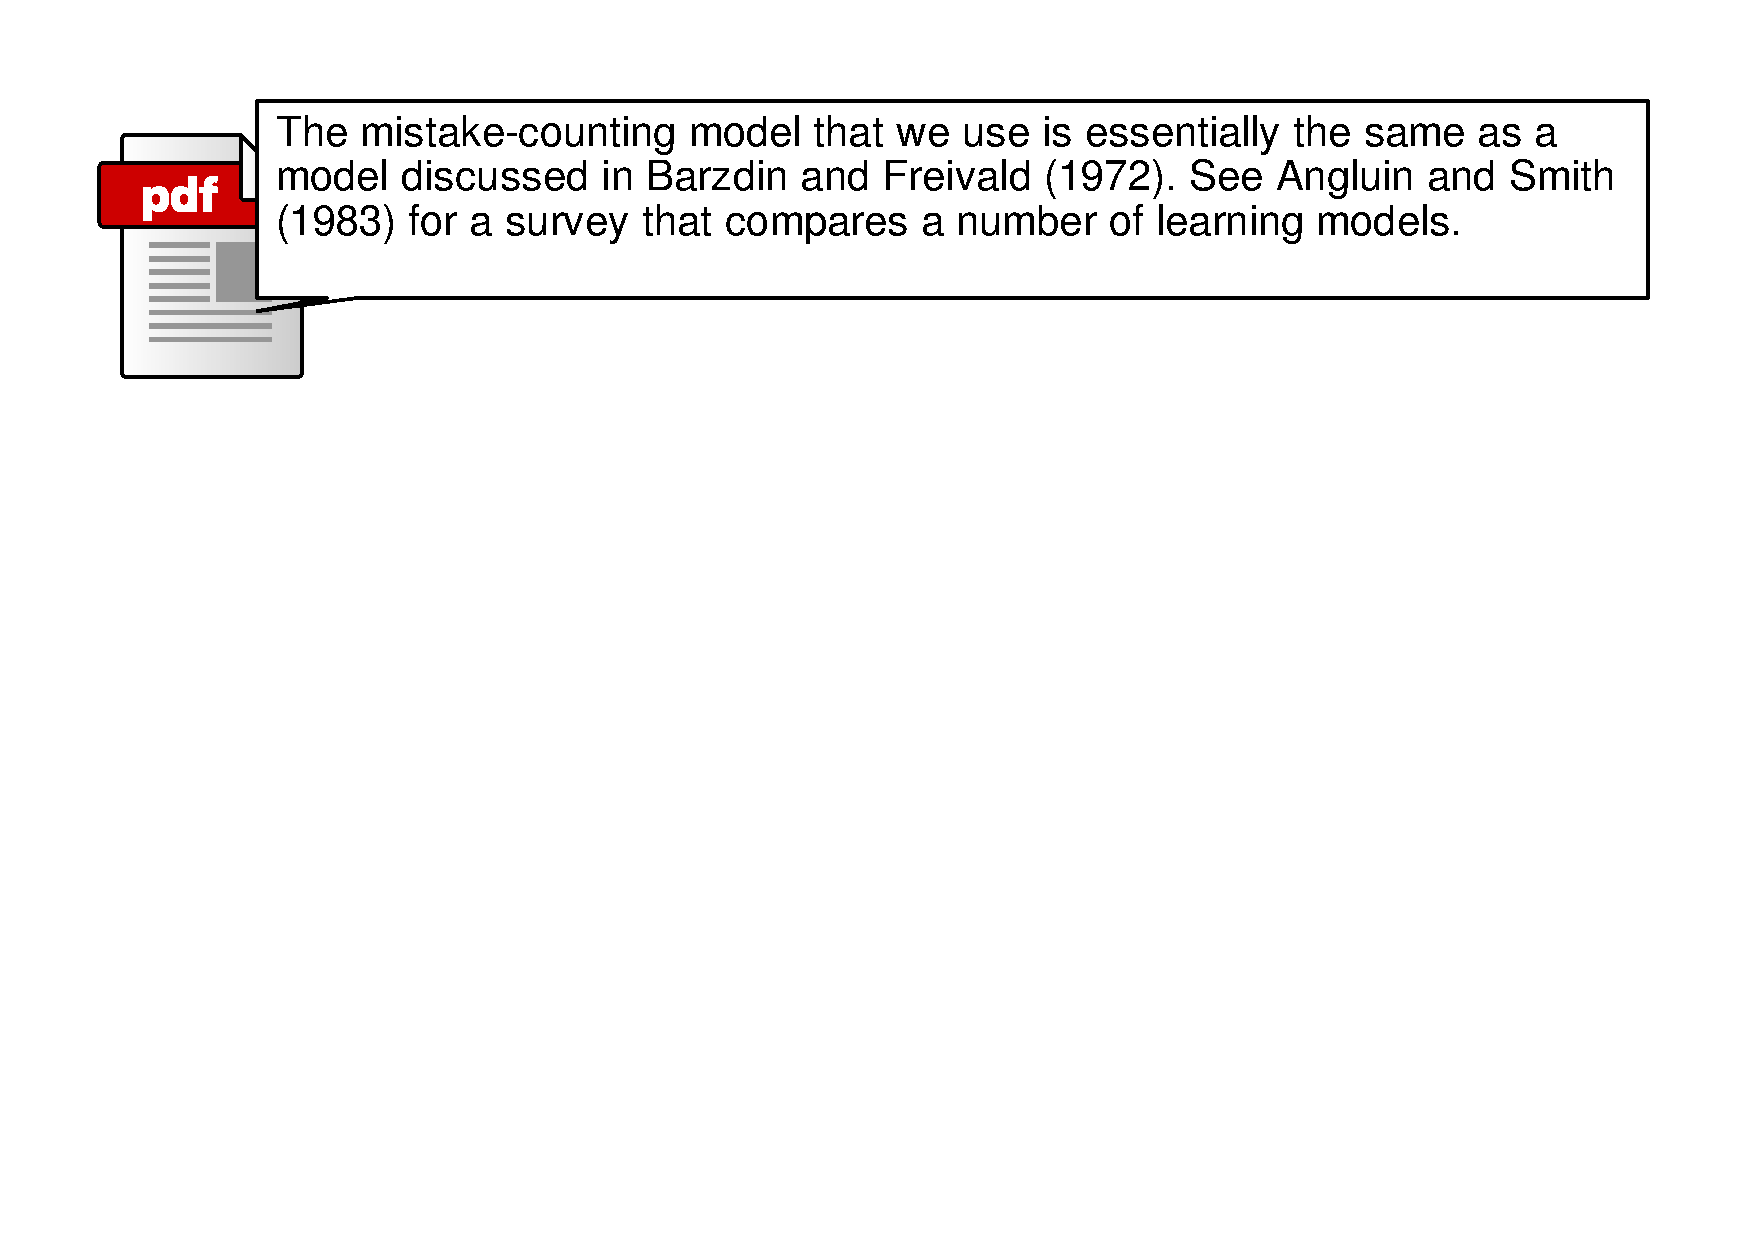
\includegraphics[scale=0.5, trim = 0mm 150mm 0mm 10mm]{no-ref-tag}
    \caption{An example of citations from the article ``Learning Abound: Quickly When Irrelevant Attributes A New Linear-threshold Algorithm'' authored by Nick Littlestone. In both sentences a link to bibliography composed from authors' names making it hard to distinguish a citation from any other sentences.} 
    \label{fig:no-ref-tag}
  \end{figure} 

Another issue in using square brackets as citation identifiers arises when square brackets are used not as links to bibliography. For example, a parser might mix up an array in a code snippet with a link to bibliography (see Figure \ref{fig:code-snippet}). Usage of code snippets are common in computer science literature so it would be nice to have a method to distinguishing a snippet of source code from the natural text. 

  \begin{figure}[htp]
    \centering
    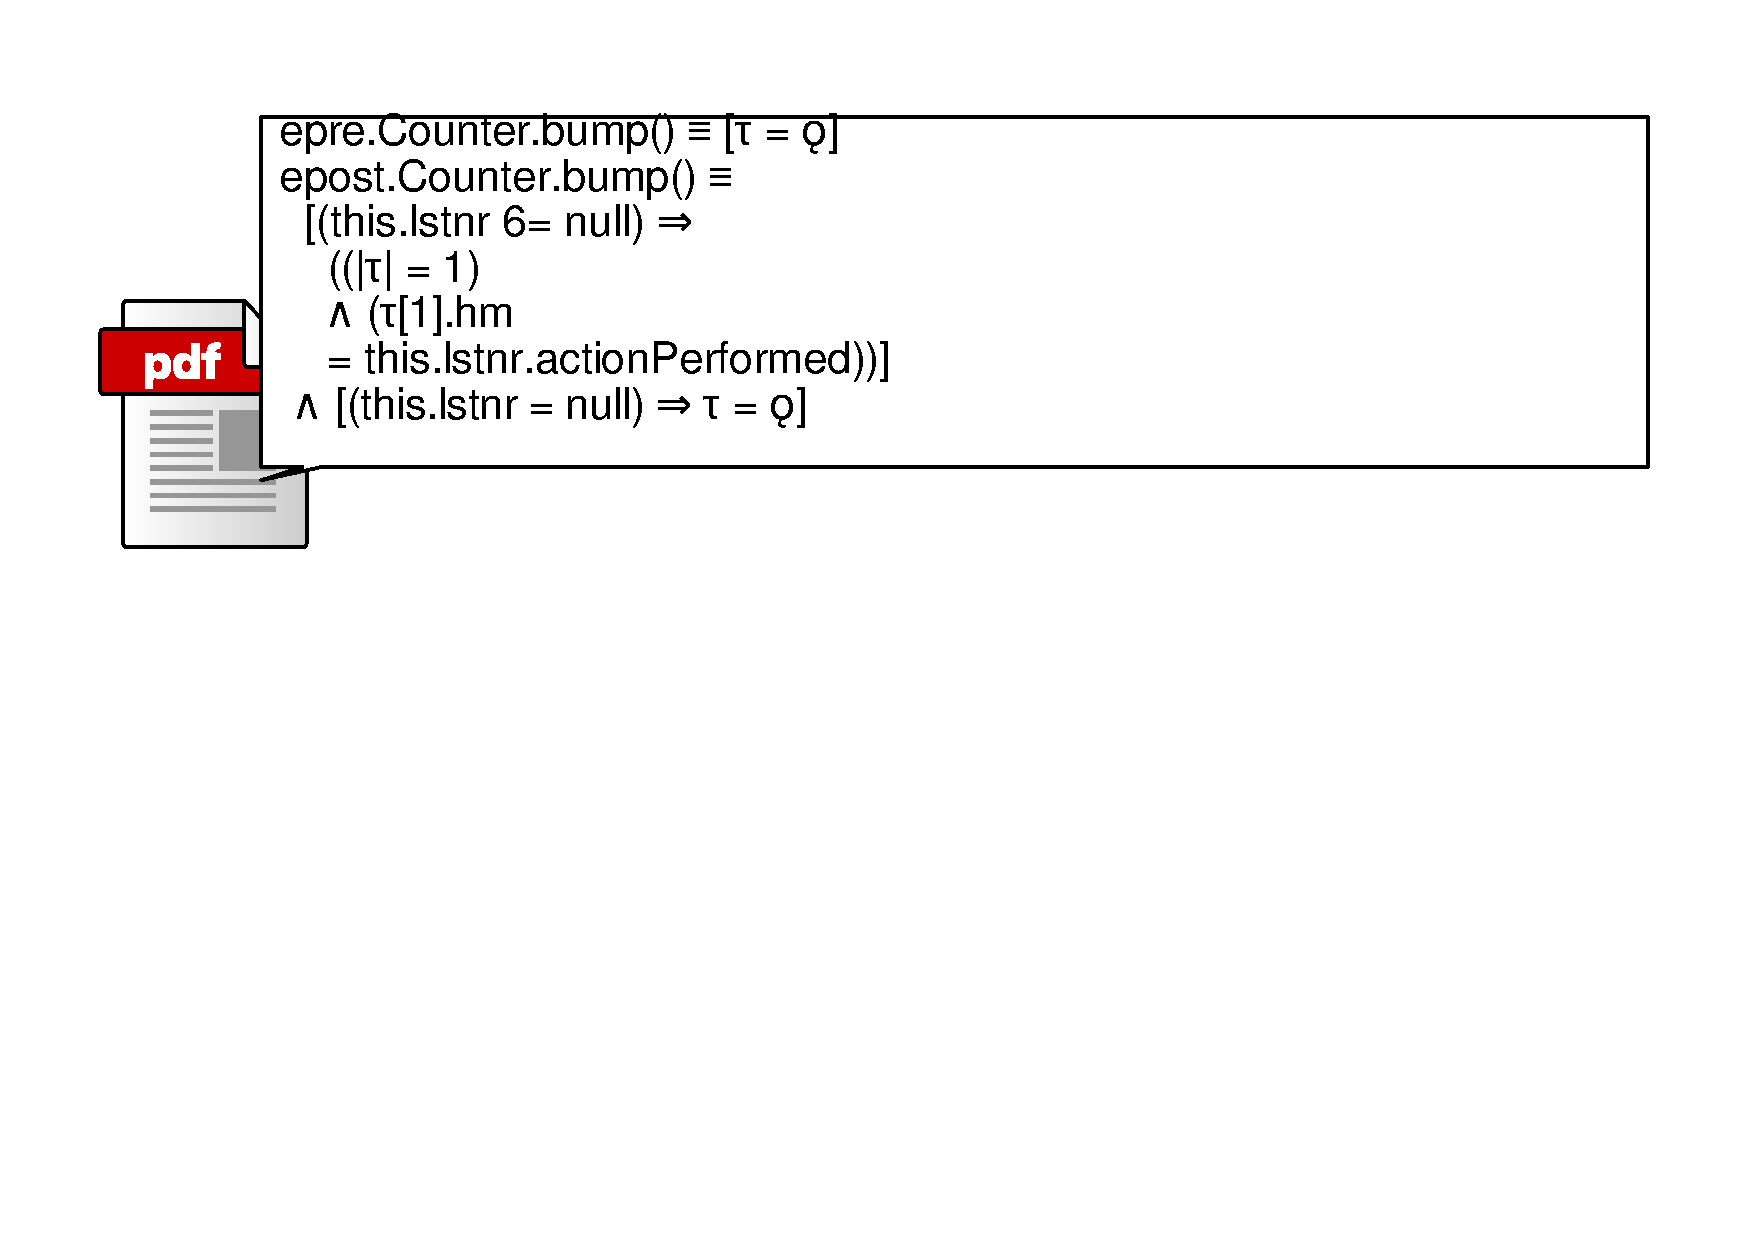
\includegraphics[scale=0.5, trim = 0mm 120mm 0mm 10mm]{code-snippet}
    \caption{An example of the code snippet from the article ``Modular Verification of Higher-Order Methods with Mandatory Calls Specified by Model Programs'' authored by Steve M. Shaner et al. The code snippet is wrongly considered as a citation and is matched to the first bibliographic entry.} 
    \label{fig:code-snippet}
  \end{figure}
  
During the debriefing interviews two participants admitted that they would like to view a title of an article from witch a citation was extracted. A title of an article could be extracted using the information about the font of the text. Such feature can be implemented using PDF parsers that provide information about the font of the extracted text.  

%END Doc
%-------------------------------------------------------

\bibliographystyle{plain}
\bibliography{thesis}

\appendix
\chapter{User Guide for CiteWise Deployment}

\section{Solr Installation}
\label{app:solr}

Solr installation requires JDK and any servlet container to be installed on the server machine. Here we describe the configuration of Solr for Apache Tomcat container.
We need to download Solr distribution that can be found on the official Solr home page \footnote{Apache Solr, \url{http://lucene.apache.org/solr/}}. Solr is distributed as an archive. After unzipping the archive, the extracts have following directories:

\begin{itemize}
	\item \textbf{contrib/} - directory containing extra libraries to Solr, such as Data Import Handler, MapReduce, Apache UIMA, Velocity Template, and so on.
	\item \textbf{dist/} - directory providing distributions of Solr and some useful libraries such as SolrJ. 
	\item \textbf{docs/} - directory with documentation for Solr.
	\item \textbf{example/} - Jetty based web application that can be used directly.
	\item \textbf{Licenses/} - directory containing all the licenses of the underlying libraries used by Solr.
\end{itemize}

Copy the dist/solr.war file from the unzipped folder to \$CATALINA\_HOME/webapps/solr.war. Then point out to Solr location of home directory describing a collection:
\begin{itemize}
	\item \textbf{Java options:} one can use following command so that the container picks up Solr collection information from the appropriate location:
	\begin{lstlisting}[language=bash]
$export JAVA_OPTS="$JAVA_OPTS -Dsolr.solr.home=/opt/solr/example"
	\end{lstlisting}
\end{itemize}
By a collection in Apache Solr one indicates a collection of Solr documents that represents one complete index.

The Solr home directory contains configuration files and index-related data. It should consist of three directories:
\begin{itemize}
\item \textbf{conf/} - directory containing configuration files, such as solrconfig.xml and schema.xml
\item \textbf{data/} - default location for storing data related to index generated by Solr
\item \textbf{lib/} - optional directory for additional libraries, used by Solr to resolve any plugins
\end{itemize}

\subsection{Solr Configuration}

Configuring Solr instance requires defining a Solr schema and configuring Solr parameters.
\paragraph{Defining Solr schema}
Solr schema is defined in the schema.xml file placed in the conf/ directory of the Solr home directory. Solr distribution comes with a sample schema file that can be changed for the needs of the project. The schema file defines the structure of the index, including fields and field types. The basic overall structure of the schema file is:
\begin{lstlisting}[language=XML]
	<schema>
	  <types>
	  <fields>
	  <uniqueKey>
	  <copyField>
	</schema>
\end{lstlisting}

The basic unit of data in Solr is document. Each document in Solr consists of fields that are described in the schema.xml file. By describing data in the schema.xml, Solr understands the structure of the data and what actions should be performed to handle this data. Here is an example of a field in the schema file:
\begin{lstlisting}[language=XML]
<field name="id" type="integer" indexed="true" stored="true" required="true"/>
\end{lstlisting}
Table \ref{tab:field.attrs} lists and explains major attributes of field element. 

\begin{table}[ht]
\begin{center}
\begin{tabular}{ | l | p{10cm}  | } 
 \hline
 Name & Description \\  \hline
 default & default value if it is not read while importing a document \\ \hline
 indexed & true if field should be indexed \\ \hline
 stored & when true a field is stored in index store and is accessible while displaying results \\ \hline
 compressed & when true a field will be zipped, applicable for text-type fields \\ \hline
 multiValued & if true, field can contain multiple values in the same document. \\ 
 \hline
\end{tabular}
\caption{Major attributes of field element in a schema.xml file}
\label{tab:field.attrs}
\end{center}
\end{table}

Here is a fragment of schema file defining fields of a document in CiteWise collection:
\begin{lstlisting}[language=XML]
    <fields>
     <field name="_version_" type="long" indexed="true" stored="true" 
     		multiValued="false"/>
     <field name="id" type="string" multiValued="false"/>
     <field name="text" type="text_en" indexed="true" multiValued="false"/>
     <field name="context" type="string" indexed="false" multiValued="false"/>
     <field name="path" type="string" indexed="false" multiValued="false"/>
     <field name="reference" type="string" indexed="false" stored="true" 
     		multiValued="true" />
    </fields>
\end{lstlisting}

Every document represents a citation with matching bibliographic references. In the schema file we indicate that we want to index a text field which is the citation text. We store an id of a citation, that is a generated value, calculated from the hash of the citation string. Specifying the id is particularly useful for updating documents. We also store a context for a citation and a path to the scientific article where the citation was found. As a citation can refer to multiple sources, we make the reference field multivalued. 

In the schema configuration file, one can define the field type, like string, date or integer and map them to Java classes. This can be handy when we define custom types. A field type includes the following information:

\begin{itemize}
\item Name
\item Implementation class name
\item If the field type is a TextField, it will include a description of the field analysis
\item Field attributes 
\end{itemize}

A sample field type description:
\begin{lstlisting}[language=XML]
	<fieldType name="text_ws" class="solr.TextField" positionIncrementGap="100">
  		<analyzer>
  		<tokenizer class="solr.WhitespaceTokenizerFactory"/>
  		</analyzer>
	</fieldType>
\end{lstlisting}

Other elements in the Solr schema file listed in Table \ref{tab:fields.others}:

\begin{table}[ht]
\begin{center}
\begin{tabular}{ | l | p{10cm}  | } 
 \hline
 Name & Description \\  \hline
 uniqueKey & specifies which field in documents is a unique identifier of a document, should be used if you ever update a document in the index\\ \hline
 copyField & used to copy field's value from one field to another \\ \hline
\end{tabular}
\caption{Description of some elements in schema.xml}
\label{tab:fields.others}
\end{center}
\end{table}

\paragraph{Configuring Solr Parameters}
To configure a Solr instance we need to describe the solrconfig.xml and solr.xml files.

\begin{description}
\item[solr.xml] The solr.xml configuration is located in solr home directory and used for configuration of logging and advanced options to run Solr in a cloud mode.
\item[solrconfig.xml] The solrconfig.xml configuration file primarily provides you with an access to index-management settings, RequestHandlers, listeners, and request dispatchers. The file has a number of complex sections and mainly is changed when a specific need is encountered. 
\end{description} 

\subsection{Enhanced Solr Search Features}
Solr provides a number of additional features that can enhance the search system. One of the features we use is synonyms. To use this feature you need to specify synonyms.txt file with listed synonyms. This file is used by synonym filter to replace words with their synonyms. For example, a search for "DVD" may expand to "DVD", "DVDs", "Digital Versatile Disk" depending on the mapping in this file. This file can be also used for spelling corrections. Here is an example of synonyms.txt file:
\begin{lstlisting}
GB, gib, gigabyte, gigabytes
MB, mib, megabyte, megabytes
Television, Televisions, TV, TVs
Incident_error, error
\end{lstlisting}

Additionally, there are other configuration files that appear in the configuration directory. We are listing them in Table \ref{tab:solr.config} with the description of each configuration:
\begin{table}[ht]
\begin{center}
\begin{tabular}{ | l | p{10cm}  | } 
 \hline
 Name & Description \\  \hline
 protwords.txt & file where you can specify protected words that you do not wish to get stemmed. So, for example, a stemmer might stem the word "catfish" to "cat" or "fish".\\ \hline
 spellings.txt & file where you can provide spelling suggestions to the end user. \\ \hline
 elevate.txt & file  where you can change the search results by making your own results among the top-ranked results. This overrides standard ranking scheme, taking into account elevations from this file. \\ \hline
 stopwords.txt & Stopwords are those that will not be indexed and used by Solr in the applications. This is particularly helpful when you really wish to get rid of certain words. For example, in the string, "Jamie and joseph," the word "and" can be marked as a stopword. \\ \hline
\end{tabular}
\caption{Additional configuration files in Solr}
\label{tab:solr.config}
\end{center}
\end{table}

\section{MongoDB Installation}
\label{app:mongo}

MongoDB is a NoSQL document-oriented database. Data in MongoDB is stored in JSON-like documents with a dynamic schema. The format of stored data is called BSON, which stands for Binary JSON. BSON is an open standard developed for human readable data exchange\footnote{BSON specification, \url{http://bsonspec.org/}}. MongoDB requires a little amount of configuration to start to work with. 

To install MonogoDB follow instruction on the official web site \url{http://docs.mongodb.org/manual/installation/}. 

\subsection{MongoDB configuration}
Once MonogDB is downloaded, it is very easy to set up a database server. All we need to start the MongoDB server is to type \emph{mongod} command. In our case we would like to specify database location with --dbpath parameter and default listening port:
\begin{lstlisting}[language=Bash]
	> mongod --dbpath /home/aliya/mongodb2 --port 27272
\end{lstlisting}

MongoDB provides REST API. To enable REST API use parameter --rest:
\begin{lstlisting}[language=Bash]
	> mongod --dbpath /home/aliya/mongodb2 --port 27272 --rest true
\end{lstlisting}

The simple way to communicate with theD MongoDB server is to use the MongoDB shell, in our case we specify --port parameter to connect to our instance of MongoDB:
\begin{lstlisting}[language=Bash]
	> mongo --port 27272
\end{lstlisting}

Compared to relational databases MongoDB operates with terms collection, which is equivalent to table, and document, which is equivalent to record in relational databases. MongoDB does not require creating databases and collections explicitly. Databases and collections can be created while starting to use MongoDB. To see list of databases or collections, type show dbs in mongo shell:
 \begin{lstlisting}[language=Bash]
	> show dbs
\end{lstlisting}
MongoDB shell allows to make queries, updates, deletes on collections, get various statistics on data and server usage, and manipulate with data with map-reduce interface, full documentation can be found on the official web site \footnote{MongoDB database, \url{http://www.mongodb.org/}}. 

\section{Running the parser}
Before running the parser Solr web application should be deployed on the Tomcat web server and MongoDB instance should be run. One should use Java version 7 or above to run the parser. Get the parser distribution:
\begin{lstlisting}[language=Bash]
	> git clone git@scg.unibe.ch:citation-search-engine
\end{lstlisting}

The cloned directory consists of three modules:
\begin{itemize}
\item \textbf{solr} - Solr related configuration files,
\item \textbf{citation\_search} - a parser of scientific articles, that extracts meta-information and publish documents to Solr and MongoDB,
\item \textbf{citation\_search\_web} - a web application for searching citations.
\end{itemize}

All files related to the parser are located in the \emph{citation\_search} directory. The \emph{citation\_search} directory has a standard Maven project layout \footnote{\href{https://maven.apache.org/guides/introduction/introduction-to-the-standard-directory-layout.html}{Apache Maven, https://maven.apache.org}}. Go to the resources \emph{parser.properties} according to your development environment. Table \ref{tab:parser-properties} describes properties of a \emph{parser.properties} file with sample values.

\begin{table}[ht]
\begin{center}
\begin{tabular}{ | l | p{4cm} | l | } 
 \hline
 \textbf{Property} & \textbf{Description} & \textbf{Sample value} \\  \hline
solr.url.citations & Endpoint for publishing citations. & http://localhost:8088/solr/collection1/\\ \hline
solr.url.bibliography & Endpoint for publishing bibliographic links. & http://localhost:8088/solr/collection2/  \\  \hline
db.host & MongoDB host server IP address. & 127.0.0.1  \\  \hline 
db.port & MongoDB listening port. & 27272  \\  \hline
db.name & MongoDB database name. & CS  \\  \hline 
db.collection & MongoDB database collection name. & papers  \\  \hline
pdfs.path & Location of pdf files. & /home/aliya/Library  \\  \hline  
\end{tabular}
\caption{Explanation of properties of a \emph{parser.properties} file.}
\label{tab:parser-properties}
\end{center}
\end{table}

One can change default logging properties for Log4j \footnote{Apache Log4j, \url{http://logging.apache.org/log4j/2.x/}} library in a \emph{logj4.properties} file.
Once property files are configured, build a jar file executing following command from the directory containing a \emph{pom.xml} file:
\begin{lstlisting}[language=Bash]
	> mvn assembly:assembly -­‐DdescriptorId=jar-­‐with-­‐dependencies –DskipTests
\end{lstlisting}

Maven will generate a jar file \emph{citation\_search-­‐1.0-­‐jar-­‐with-­‐dependencies.jar} in a \emph{target} folder. To execute the jar file run following command:
\begin{lstlisting}[language=Bash]
	> java -­‐jar citation_search-­‐1.0-­‐jar-­‐with-­‐dependencies.jar
\end{lstlisting}

\section{Search Interface Deployment}

All web application related web files are located in a \emph{citation\_search\_web} directory. The directory has a standard Maven project layout \footnote{\href{https://maven.apache.org/guides/introduction/introduction-to-the-standard-directory-layout.html}{Apache Maven, https://maven.apache.org}}. Change a \emph{search.properties} file in a \emph{resources} folder. Table \ref{tab:search-properties} describes properties of a \emph{search.properties} file with sample values . 

\begin{table}[ht]
\begin{center}
\begin{tabular}{ | l | p{4cm} | l | } 
 \hline
 \textbf{Property} & \textbf{Description} & \textbf{Sample value} \\  \hline
solr.url.citations & Endpoint for querying citations. & http://localhost:8088/solr/collection1/\\ \hline
solr.url.bibliography & Endpoint for querying bibliographic links. & http://localhost:8088/solr/collection2/  \\  \hline
\end{tabular}
\caption{Explanation of properties of a \emph{search.properties} file.}
\label{tab:search-properties}
\end{center}
\end{table}

One can change default logging properties for Log4j \footnote{Apache Log4j, \url{http://logging.apache.org/log4j/2.x/}} library in a \emph{logj4.properties} file.
Once property files are configured, build a war file executing following command from the directory containing a \emph{pom.xml} file:
\begin{lstlisting}[language=Bash]
	> mvn package -­‐DskipTests
\end{lstlisting}

Maven will generate a war file in a \emph{target} folder. Deploy to the Tomcat web server by putting a war­‐file in a Tomcat \emph{webapp} directory or use a Tomcat web interface to deploy through Tomcat's manager. 


\end{document}